\documentclass[12pt,a4paper]{article}

\usepackage[italian]{babel}
\usepackage[T1]{fontenc}
\usepackage[utf8]{inputenc}
\usepackage{lmodern}
\usepackage{geometry}
\usepackage{setspace}
\usepackage{graphicx}
\usepackage{float}
\usepackage{hyperref}
\usepackage{booktabs}
\usepackage[table]{xcolor}
\usepackage{listings}
\usepackage{caption}
\usepackage{subcaption}
\usepackage{enumitem}
\usepackage{longtable}
\usepackage{array}
\usepackage{microtype}
\usepackage{fancyhdr}

\geometry{margin=2.4cm}
\onehalfspacing
\setlength{\emergencystretch}{3em}
\graphicspath{{img/}}
\hypersetup{
  colorlinks=true,
  linkcolor=blue!55!black,
  urlcolor=blue!65!black,
  citecolor=blue!55!black,
  pdftitle={DineUp/YouDine - Relazione di Ingegneria del Software},
  pdfauthor={Francesco Cinotti e Leonardo Panizzi}
}

\pagestyle{fancy}
\fancyhf{}
\fancyhead[L]{DineUp}
\fancyhead[R]{Ingegneria del Software}
\fancyfoot[C]{\thepage}
\setlength{\headheight}{15pt}

\definecolor{codebg}{RGB}{247,248,250}
\definecolor{codeframe}{RGB}{190,198,205}
\lstdefinestyle{codeStyle}{
  basicstyle=\ttfamily\footnotesize,
  backgroundcolor=\color{codebg},
  breaklines=true,
  frame=single,
  rulecolor=\color{codeframe},
  tabsize=2,
  numbers=left,
  numberstyle=\tiny\color{gray},
  keywordstyle=\color{blue!70!black},
  commentstyle=\color{green!40!black},
  stringstyle=\color{orange!70!black},
  showstringspaces=false,
  columns=fullflexible
}

\newcommand{\project}{\textbf{DineUp}}
\newcommand{\code}[1]{\nolinkurl{#1}}
\newcommand{\HRule}{\rule{\linewidth}{0.5mm}}

\title{
  \vspace{1.5cm}
  {\Huge\textbf{DineUp}}\\[0.4cm]
  {\Large Sistema console per la gestione di un ristorante}\\[1.5cm]
  {\large Relazione di Ingegneria del Software}
}
\author{
  Francesco Cinotti\\
  Corso di Laurea in Ingegneria Informatica\\
  Università degli Studi di Firenze
}
\date{Anno Accademico 2025--2026}

\begin{document}

\begin{titlepage}
\newgeometry{top=2.5cm,bottom=2.5cm,left=3cm,right=3cm}
\thispagestyle{empty}
\begin{center}

\IfFileExists{mokup/logounifi.png}{
  
\includegraphics[width=0.48\textwidth]{mokup/logounifi.png}\\[0.6cm]
}{
  \vspace*{1.2cm}
}

\textsc{\LARGE Università degli Studi di Firenze}\\[0.45cm]
\textsc{\Large Dipartimento di Ingegneria dell'Informazione}\\[1.2cm]

\HRule\\[0.8cm]
{\Huge\bfseries DineUp/YouDine}\\[0.35cm]
{\Large Sistema gestionale per attività di ristorazione}\\[0.8cm]
\HRule\\[1.6cm]

\begin{minipage}[t]{0.46\textwidth}
  \begin{flushleft}\large
    \emph{Autori:}\\
    Francesco Cinotti\\
    Leonardo Panizzi\\[1.2em]
    \emph{N\textsuperscript{o} matricola:}\\
    7077005\\
    7077368
  \end{flushleft}
\end{minipage}
\hfill
\begin{minipage}[t]{0.46\textwidth}
  \begin{flushright}\large
    \emph{Corso:}\\
    Ingegneria del Software\\[1.2em]
    \emph{Docente del corso:}\\
    Prof.\ Enrico Vicario
  \end{flushright}
\end{minipage}

\vfill
{\large Anno Accademico 2025--2026}

\end{center}
\restoregeometry
\end{titlepage}

\newpage

\tableofcontents
\newpage

\section{Introduzione}

\subsection{Contesto e motivazioni}

\project{} è un'applicazione Java a riga di comando per la gestione delle principali
attività di un ristorante. Il software nasce dall'esigenza di coordinare, in un unico
sistema, il lavoro del cliente, dello staff operativo e del proprietario. Il dominio
comprende la consultazione del menu, gli ordini d'asporto, le prenotazioni dei tavoli,
la gestione delle fasce orarie, le notifiche e l'amministrazione delle risorse del locale.

Il progetto non si limita a fornire operazioni CRUD sul database. La parte centrale è
costituita dalle regole di dominio: transizioni ammesse per ordini e prenotazioni,
allocazione dei tavoli, prevenzione delle doppie prenotazioni, costruzione dinamica dei
criteri di ricerca e separazione delle responsabilità tra interfaccia, logica applicativa
e persistenza.

\subsection{Obiettivi}

Gli obiettivi principali sono:

\begin{itemize}[leftmargin=*]
  \item modellare un dominio realistico mediante entità, value object ed enumerazioni;
  \item fornire funzionalità differenti per i ruoli \emph{Customer}, \emph{Staff} e
        \emph{Owner};
  \item separare la presentazione CLI dalla logica applicativa e dall'accesso ai dati;
  \item garantire la consistenza di ordini e prenotazioni mediante transazioni;
  \item supportare ricerche componibili senza moltiplicare i metodi specializzati;
  \item verificare il comportamento con test unitari, test dei controller e test di
        integrazione DAO su PostgreSQL.
\end{itemize}

\subsection{Tecnologie e strumenti}

\begin{table}[H]
\centering
\rowcolors{2}{gray!8}{white}
\begin{tabular}{p{4.1cm}p{10cm}}
\toprule
\textbf{Tecnologia} & \textbf{Impiego nel progetto} \\
\midrule
Java 17 & Implementazione dell'applicazione e del Domain Model. \\
Maven & Gestione delle dipendenze, compilazione ed esecuzione della suite di test. \\
PostgreSQL & Persistenza relazionale, vincoli, trigger e transazioni. \\
PostgreSQL JDBC 42.7.8 & Comunicazione tra DAO e database. \\
jBCrypt 0.4 & Hashing e verifica delle password. \\
JUnit Jupiter 5.11.4 & Test unitari e di integrazione. \\
StarUML & Modellazione dei diagrammi UML. \\
Git e GitHub & Versionamento del codice e repository del progetto. \\
\bottomrule
\end{tabular}
\caption{Tecnologie principali.}
\end{table}

\section{Analisi dei requisiti}

\subsection{Attori}

\begin{description}[leftmargin=3.2cm,style=nextline]
  \item[Customer] può registrarsi e autenticarsi, consultare e cercare il menu,
  gestire il carrello, creare un ordine d'asporto, effettuare o annullare una
  prenotazione, modificare il profilo e consultare le notifiche.

  \item[Staff] controlla la coda della cucina, aggiorna lo stato degli ordini,
  consulta e ricerca le prenotazioni, conferma l'arrivo del cliente, registra
  check-in o no-show e gestisce le notifiche operative.

  \item[Owner] amministra categorie, piatti, tavoli e slot; consulta il riepilogo
  del menu, esegue ricerche su piatti, ordini e prenotazioni e gestisce le proprie
  notifiche.
\end{description}

\subsection{Casi d'uso del Customer}

\begin{figure}[H]
  \centering
  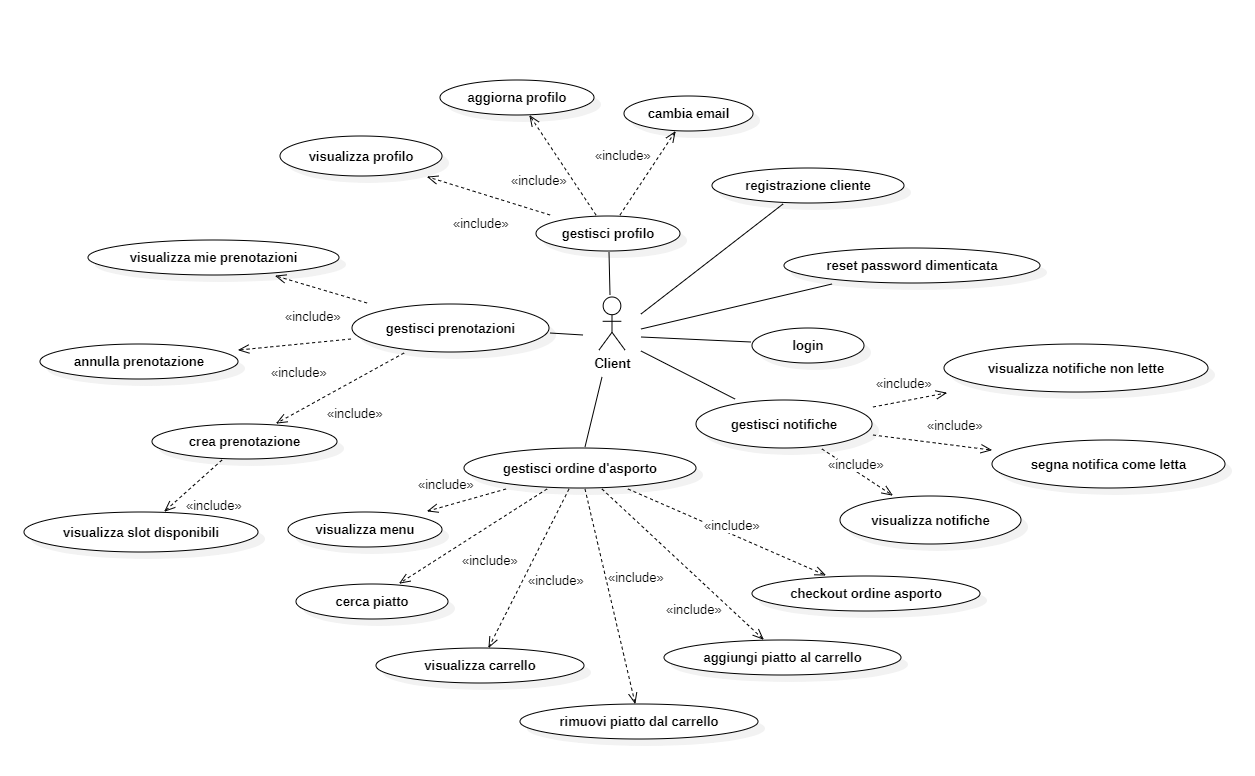
\includegraphics[width=\textwidth]{uml-usecase-client.png}
  \caption{Use Case Diagram del Client realizzato in StarUML.}
  \label{fig:uc-customer}
\end{figure}

Il flusso più articolato è quello dell'ordine d'asporto. Il cliente consulta il
menu, seleziona i piatti, modifica le quantità e conclude l'operazione scegliendo
il metodo di pagamento. Il carrello è mantenuto in memoria dal
\code{CartService}; al checkout viene trasformato in un ordine persistente e,
solo dopo il salvataggio, viene svuotato.

\subsection{Casi d'uso dello Staff}

\begin{figure}[H]
  \centering
  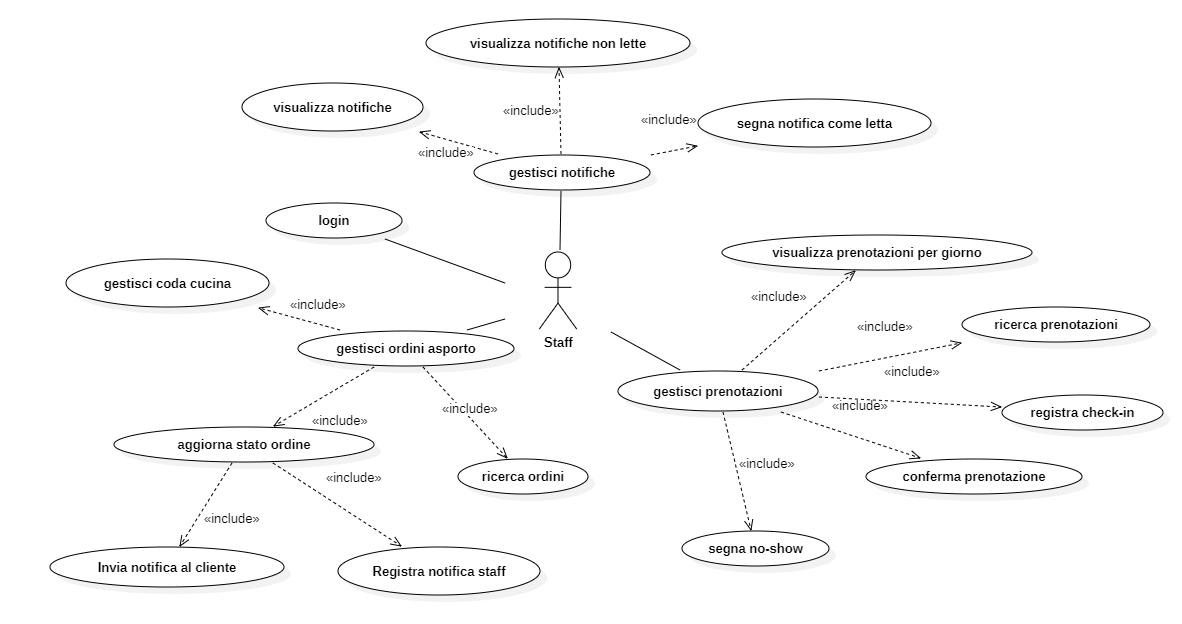
\includegraphics[width=\textwidth]{uml-usecase-staff.png}
  \caption{Use Case Diagram dello Staff realizzato in StarUML.}
  \label{fig:uc-staff}
\end{figure}

Lo Staff gestisce il ciclo operativo dell'ordine:
\code{CREATED}, \code{PREPARING}, \code{READY}, \code{RETIRED} oppure
\code{CANCELLED}. Le transizioni sono validate dal Domain Model. L'aggiornamento
produce inoltre una notifica per il cliente e una registrazione destinata
all'operatore che ha compiuto l'azione.

\subsection{Casi d'uso dell'Owner}

\begin{figure}[H]
  \centering
  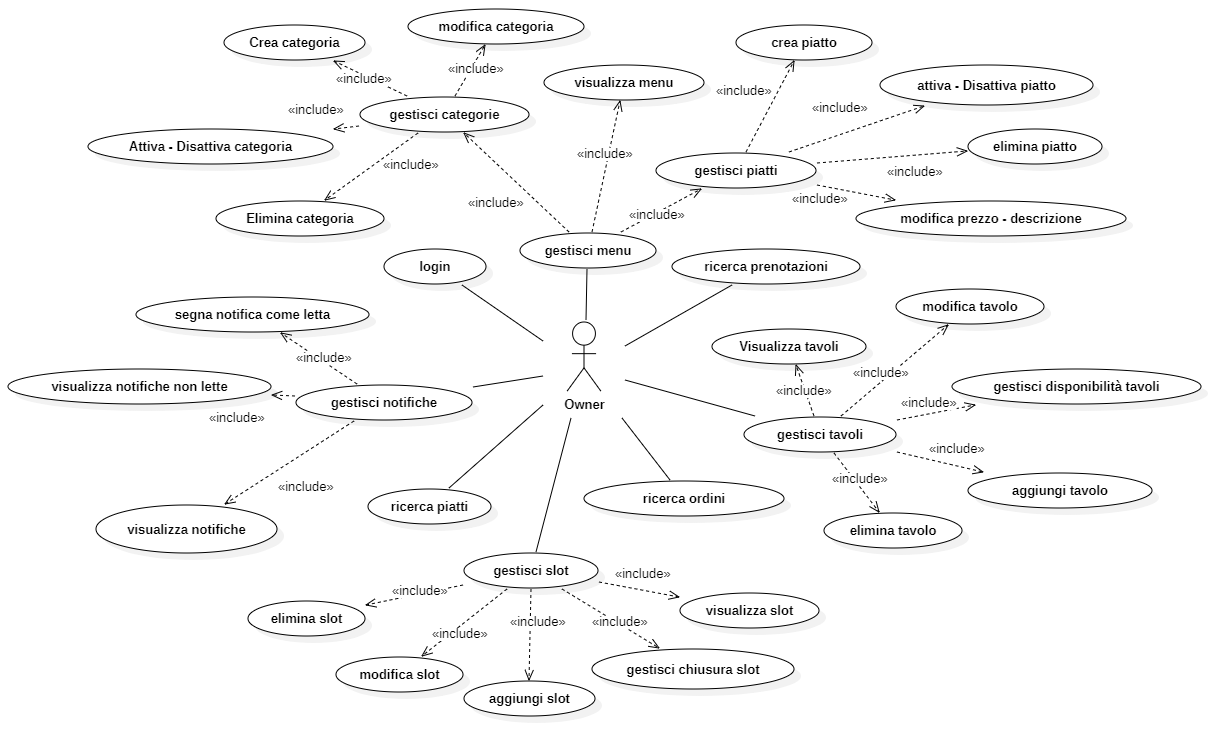
\includegraphics[width=\textwidth]{uml-usecase-owner.png}
  \caption{Use Case Diagram dell'Owner realizzato in StarUML.}
  \label{fig:uc-owner}
\end{figure}

L'Owner dispone delle operazioni amministrative sul menu e sulle risorse fisiche
del ristorante. L'eliminazione è affiancata da operazioni di attivazione e
disattivazione, utili per nascondere temporaneamente categorie, piatti, tavoli o
slot senza perdere i dati storici.

\subsection{Template dei casi d'uso principali}

\begingroup
\setlength{\arrayrulewidth}{0.3pt}
\setlength{\LTleft}{0.55cm}
\setlength{\LTright}{0.55cm}
\renewcommand{\arraystretch}{1.12}

\begin{longtable}{|>{\bfseries}p{3cm}|p{10.5cm}|}
\caption{UC1 -- Checkout ordine d'asporto.}\label{tab:uc-checkout}\\
\hline
Nome & Checkout ordine d'asporto \\
\hline
Attore & Customer autenticato. \\
\hline
Precondizioni & Il carrello contiene almeno un piatto; il cliente è persistito nel sistema. \\
\hline
Flusso principale &
Il cliente visualizza il riepilogo, sceglie il metodo di pagamento e conferma.
Il Controller recupera gli elementi dal carrello e delega la creazione
dell'ordine al Service Layer. Il DAO salva ordine e righe nella stessa
transazione. A operazione conclusa il carrello viene svuotato. \\
\hline
Flussi alternativi &
Carrello vuoto; dati del cliente non validi; errore SQL durante il salvataggio.
In caso di errore la transazione viene annullata e il carrello non viene perso. \\
\hline
Postcondizioni & Ordine e righe risultano persistiti in modo atomico. \\
\hline
\end{longtable}

\begin{longtable}{|>{\bfseries}p{3cm}|p{10.5cm}|}
\caption{UC2 -- Creazione prenotazione.}\label{tab:uc-reservation}\\
\hline
Nome & Creazione prenotazione con allocazione tavoli \\
\hline
Attore & Customer autenticato. \\
\hline
Precondizioni & Data inserita, slot esistente e aperto, numero di ospiti positivo. \\
\hline
Flusso principale &
Il sistema recupera lo slot e i tavoli disponibili, esclude quelli già assegnati
e calcola la combinazione migliore. Prenotazione e assegnazioni vengono inserite
nella stessa transazione; il cliente riceve una notifica di conferma. \\
\hline
Flussi alternativi &
Slot inesistente o chiuso; nessuna combinazione sufficiente; tavolo assegnato
contemporaneamente da un'altra richiesta. \\
\hline
Postcondizioni & Prenotazione e tavoli assegnati sono coerenti oppure non viene salvato nulla. \\
\hline
\end{longtable}

\begin{longtable}{|>{\bfseries}p{3cm}|p{10.5cm}|}
\caption{UC3 -- Aggiornamento dello stato di un ordine.}\label{tab:uc-order-status}\\
\hline
Nome & Aggiornamento stato ordine \\
\hline
Attore & Staff autenticato. \\
\hline
Precondizioni & L'ordine esiste e la transizione richiesta è ammessa. \\
\hline
Flusso principale &
Lo Staff seleziona ordine e nuovo stato. Il servizio carica l'ordine, applica
la transizione di dominio, aggiorna il database e genera le notifiche. \\
\hline
Flussi alternativi &
Ordine inesistente; transizione illegale, ad esempio da \code{RETIRED} a
\code{PREPARING}; errore di persistenza. \\
\hline
Postcondizioni & Stato aggiornato e notifiche disponibili agli utenti interessati. \\
\hline
\end{longtable}

\begin{longtable}{|>{\bfseries}p{3cm}|p{10.5cm}|}
\caption{UC4 -- Autenticazione e instradamento per ruolo.}\label{tab:uc-login}\\
\hline
Nome & Autenticazione utente \\ 
\hline
Attore & Utente registrato con ruolo Customer, Staff oppure Owner. \\
\hline
Precondizioni & L'utente possiede un account persistito e inserisce email e password. \\
\hline
Flusso principale &
L'utente immette le credenziali. Il Controller delega ad
\code{AuthService}, che recupera l'utente tramite \code{UserDAO} e verifica la
password con BCrypt. Se le credenziali sono valide, \code{Main} legge il ruolo e
avvia la CLI corrispondente: \code{CustomerCLI}, \code{StaffCLI} oppure
\code{OwnerCLI}. \\
\hline
Flussi alternativi &
Email o password vuote; utente inesistente; password errata; indisponibilità del
database. Nei primi tre casi l'accesso viene negato senza rivelare quale
credenziale sia errata. \\
\hline
Postcondizioni & L'utente autenticato accede esclusivamente alle funzionalità previste dal proprio ruolo. \\
\hline
\end{longtable}

\begin{longtable}{|>{\bfseries}p{3cm}|p{10.5cm}|}
\caption{UC5 -- Gestione operativa di una prenotazione.}\label{tab:uc-reservation-operation}\\
\hline
Nome & Conferma, check-in o registrazione del no-show \\
\hline
Attore & Staff autenticato. \\
\hline
Precondizioni & La prenotazione esiste e si trova in uno stato compatibile con l'operazione richiesta. \\
\hline
Flusso principale &
Lo Staff ricerca o visualizza le prenotazioni della giornata e seleziona
l'operazione. Il Controller delega a \code{StaffOperationService} e
\code{ReservationService}; il Domain Model applica la transizione, il DAO
aggiorna lo stato e viene generata una notifica per il Customer. \\
\hline
Flussi alternativi &
Prenotazione inesistente; transizione non ammessa, ad esempio check-in di una
prenotazione non confermata; errore durante l'aggiornamento o il salvataggio
della notifica. \\
\hline
Postcondizioni & Lo stato della prenotazione è aggiornato e l'evento operativo risulta disponibile al sistema. \\
\hline
\end{longtable}

\newpage
\begin{table}[H]
\centering
\caption{UC6 -- Gestione di un piatto del menu.}
\label{tab:uc-dish-management}
\begin{tabular}{|>{\bfseries}p{3cm}|p{10.5cm}|}
\hline
Nome & Creazione e amministrazione di un piatto \\
\hline
Attore & Owner autenticato. \\
\hline
Precondizioni & Per la creazione esiste una categoria valida; per modifica,
attivazione o eliminazione il piatto è già presente. \\
\hline
Flusso principale &
L'Owner seleziona l'operazione desiderata. Per la creazione inserisce nome,
descrizione, prezzo e categoria. Il Controller costruisce un \code{Money} e
delega a \code{OwnerAdminService}, che recupera la categoria e persiste il
piatto tramite \code{DishDAO}. Le operazioni successive consentono di aggiornare
prezzo o descrizione, modificare la disponibilità oppure eliminare il piatto. \\
\hline
Flussi alternativi &
Nome assente; prezzo negativo; categoria o piatto inesistente; violazione di un
vincolo del database; errore di persistenza. \\
\hline
Postcondizioni & Il menu persistito riflette la creazione o la modifica richiesta; un piatto disattivato non è proposto al Customer. \\
\hline
\end{tabular}
\end{table}

\endgroup

\section{Architettura software}

\subsection{Architettura a layer}

\begin{figure}[H]
  \centering
  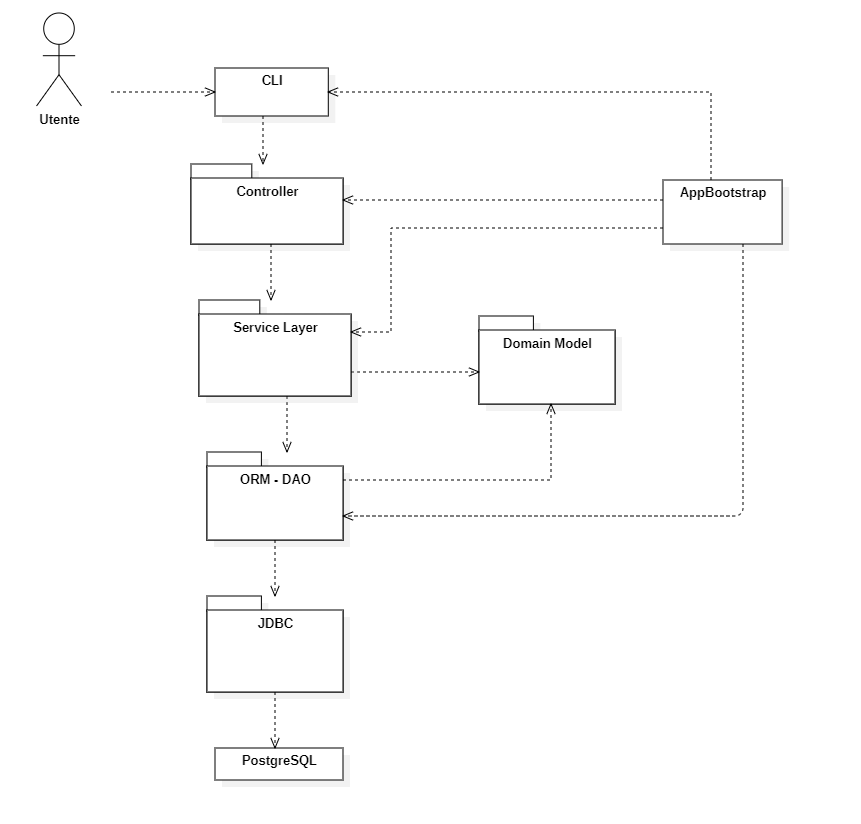
\includegraphics[width=0.72\textwidth]{uml-package.png}
  \caption{Package Diagram dell'architettura applicativa.}
  \label{fig:architecture}
\end{figure}

L'architettura applica una separazione a livelli:

\begin{itemize}[leftmargin=*]
  \item la \textbf{CLI} legge input e presenta risultati ed errori;
  \item i \textbf{Controller} espongono i casi d'uso alla CLI e coordinano i servizi;
  \item il \textbf{Service Layer} contiene le regole applicative;
  \item il \textbf{Domain Model} rappresenta stato e comportamento del dominio;
  \item i \textbf{DAO} isolano query, mapping e transazioni;
  \item JDBC collega il programma a PostgreSQL.
\end{itemize}

La scelta di rimuovere le stampe dai Controller rende la logica riutilizzabile e
facilita i test: un Controller restituisce oggetti o collezioni e la formattazione
rimane responsabilità esclusiva della CLI.

\subsection{Composition Root}

\code{AppBootstrap} costituisce il punto unico di composizione. Crea prima i DAO,
poi i servizi, quindi i Controller e infine le CLI. In questo modo le dipendenze
sono esplicite e non vengono istanziate in punti imprevedibili del codice.

\begin{lstlisting}[style=codeStyle,language=Java,
caption={Composizione esplicita dei componenti.}]
MenuQueryService menu =
    new MenuQueryService(dishDAO, categoryDAO);
OrderService orders = new OrderService(orderDAO);
ReservationService reservations = new ReservationService(
    reservationDAO, tableDAO, slotDAO,
    notificationDAO, tableAllocationService);

CustomerController customer = new CustomerController(
    menu, cartService, orders, reservations, notificationService);
\end{lstlisting}

\subsection{Responsabilità dei package}

\begin{table}[H]
\centering
\rowcolors{2}{gray!8}{white}
\begin{tabular}{p{3.2cm}p{10.7cm}}
\toprule
\textbf{Package} & \textbf{Responsabilità} \\
\midrule
\code{CLI} & Menu testuali, acquisizione input, stampa di risultati ed errori. \\
\code{Controller} & API dei casi d'uso per ciascun ruolo. \\
\code{ServiceLayer} & Regole di business, transizioni, ricerche e notifiche. \\
\code{DomainModel} & Entità, enumerazioni, value object e parametri di ricerca. \\
\code{ORM} & DAO, connessione, mapping JDBC e migrazioni. \\
\bottomrule
\end{tabular}
\caption{Suddivisione delle responsabilità.}
\end{table}

\subsection{Diagrammi delle classi per layer}

I diagrammi sono riportati integralmente, senza suddivisioni, per preservare
la visione d'insieme delle classi e delle dipendenze tra i layer. Ogni package
è presentato su una pagina verticale dedicata, secondo l'impostazione adottata
nelle relazioni prese come riferimento.

\begin{figure}[H]
  \centering
  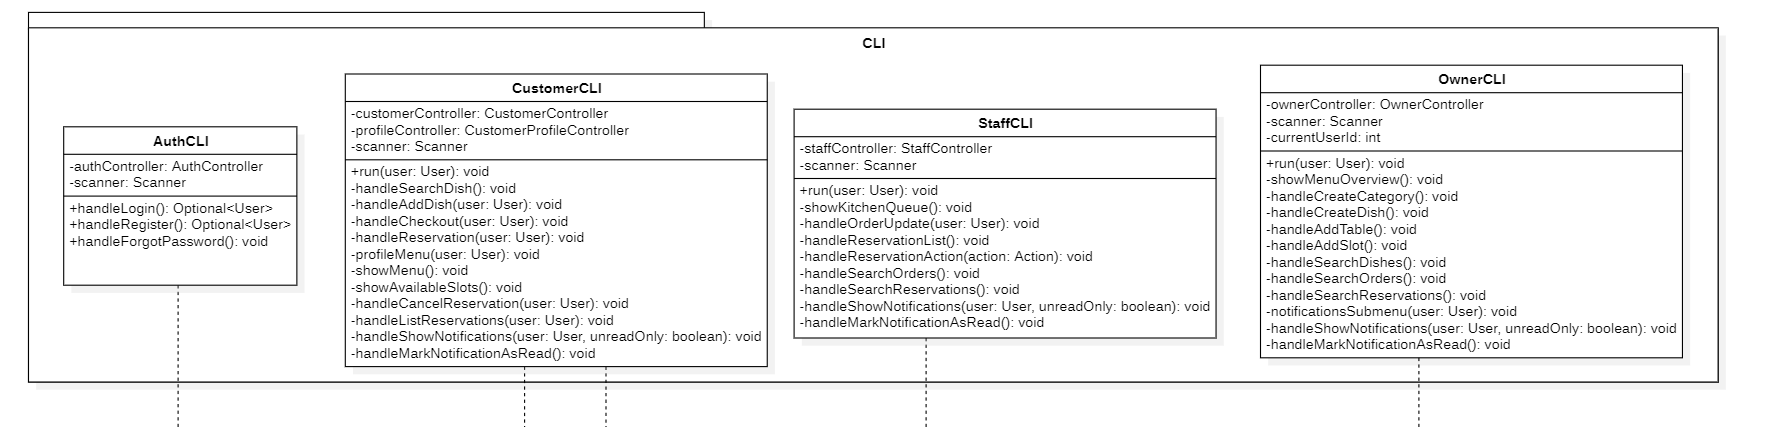
\includegraphics[width=\textwidth,height=0.76\textheight,keepaspectratio]{uml-cli.png}
  \caption{Diagramma completo del package CLI.}
\end{figure}

\begin{figure}[H]
  \centering
  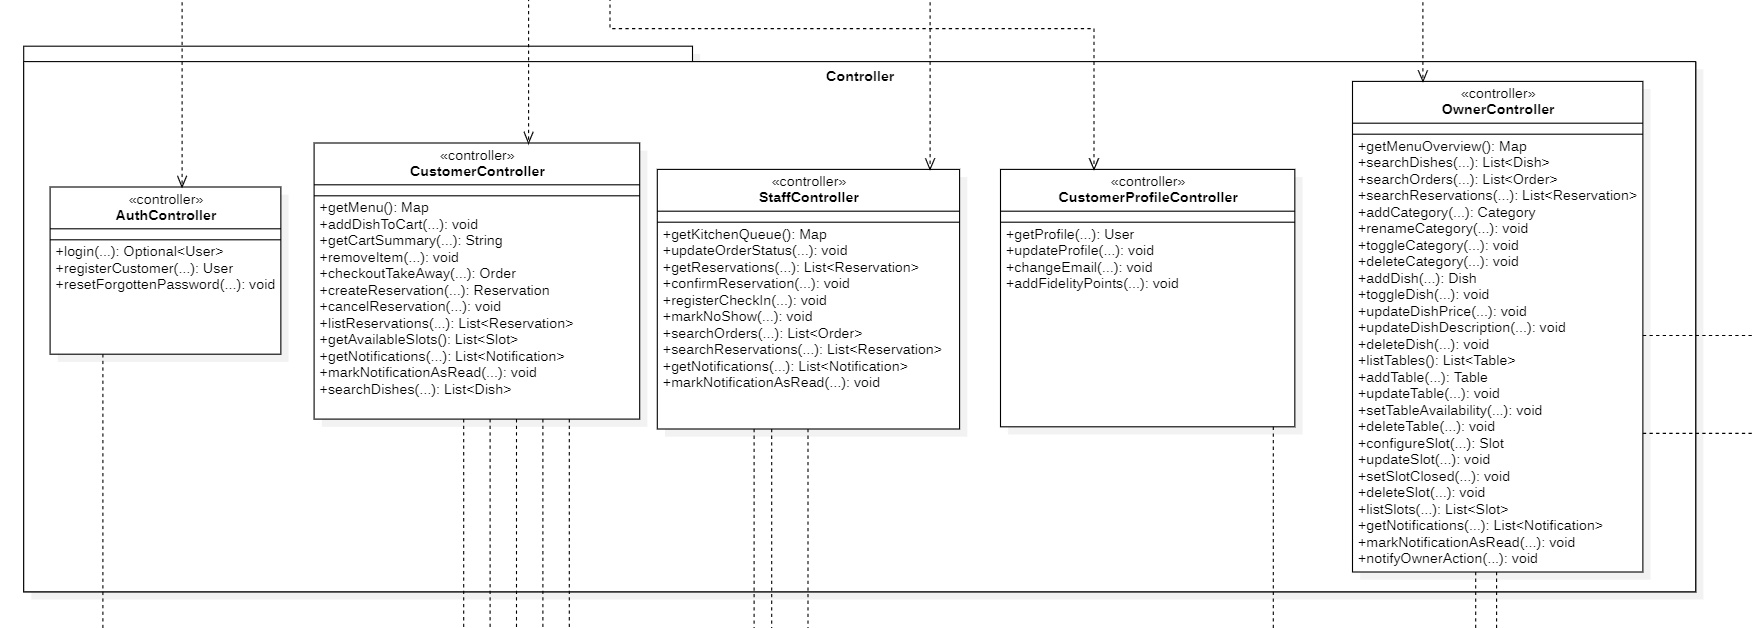
\includegraphics[width=\textwidth,height=0.76\textheight,keepaspectratio]{uml-controller.png}
  \caption{Diagramma completo del package Controller.}
\end{figure}

\begin{figure}[H]
  \centering
  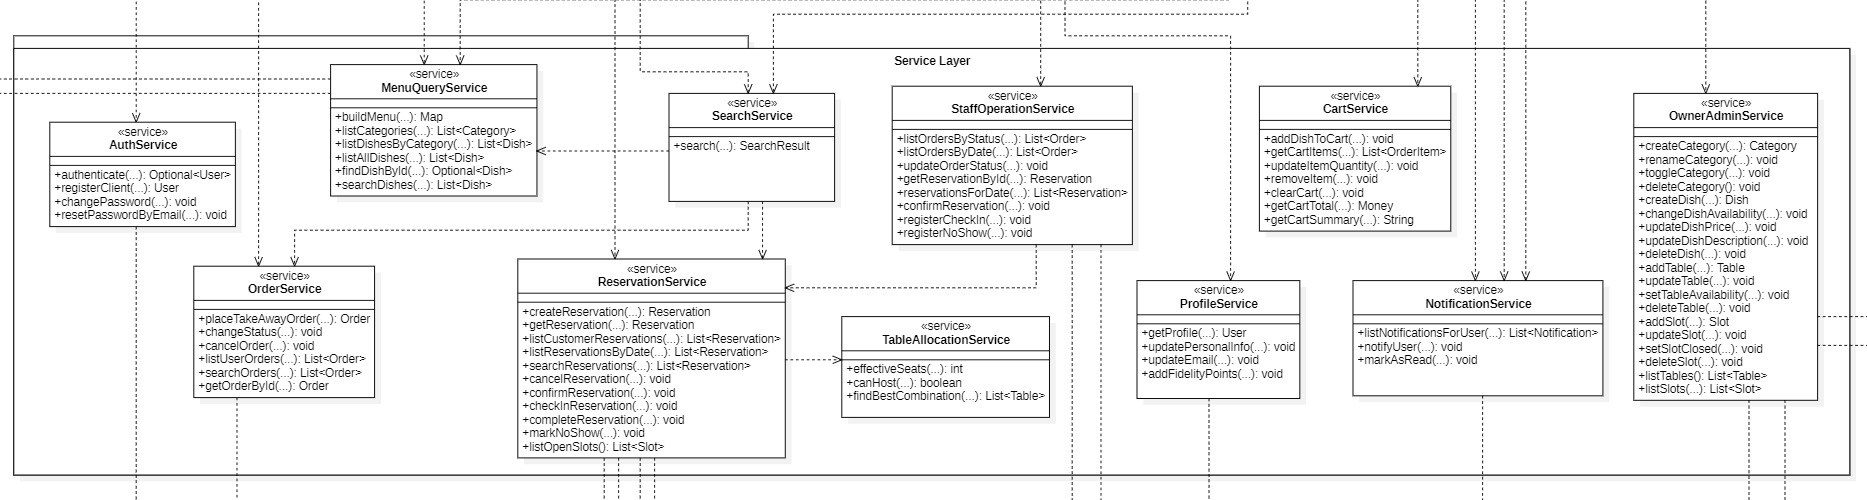
\includegraphics[width=\textwidth,height=0.76\textheight,keepaspectratio]{uml-service.png}
  \caption{Diagramma completo del Service Layer.}
\end{figure}

\begin{figure}[H]
  \centering
  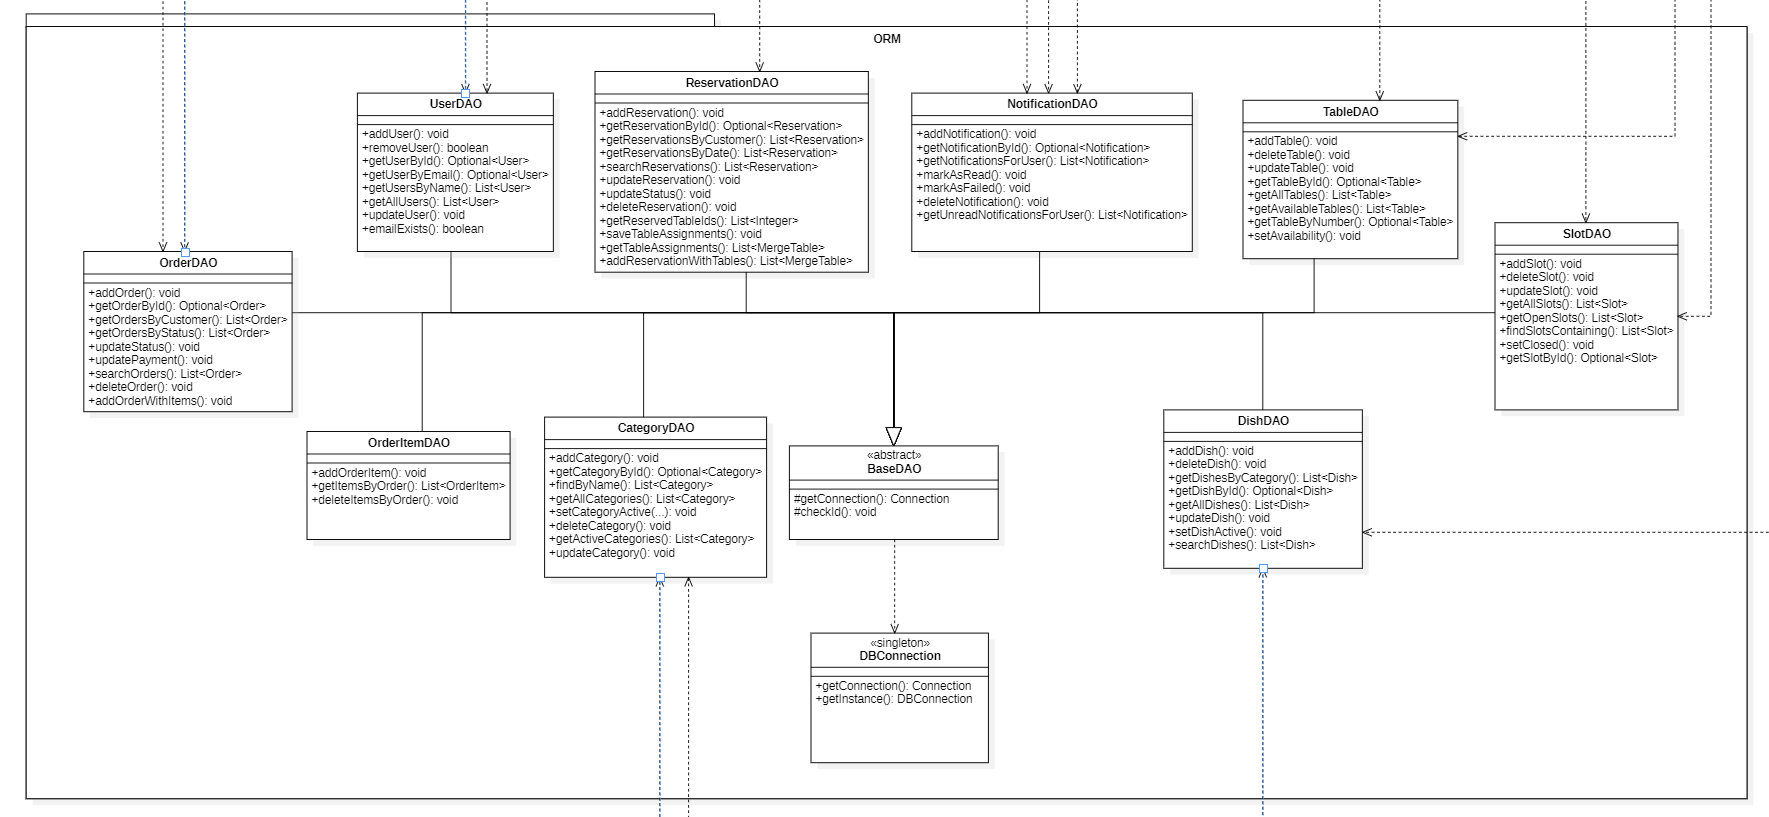
\includegraphics[width=\textwidth,height=0.76\textheight,keepaspectratio]{uml-orm.png}
  \caption{Diagramma completo del package ORM/DAO.}
\end{figure}

\section{Progettazione del Domain Model}

\subsection{Organizzazione}

\begin{figure}[H]
  \centering
  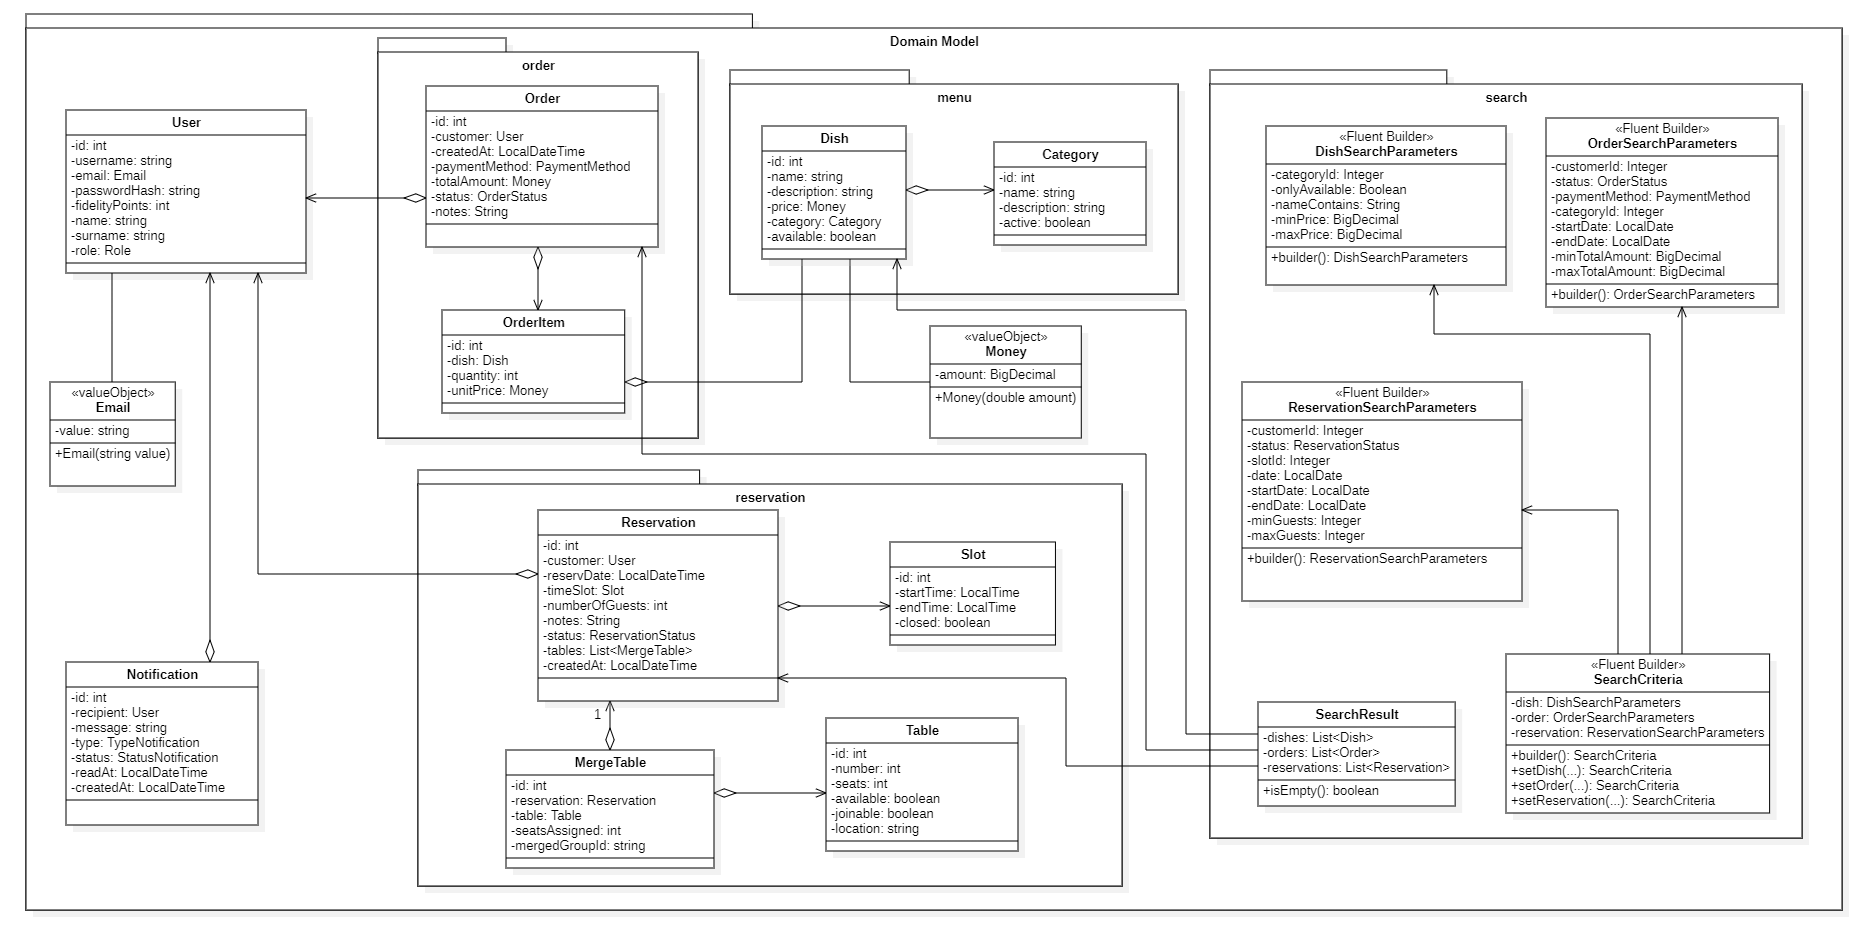
\includegraphics[width=\textwidth,height=0.76\textheight,keepaspectratio]{uml-domain.png}
  \caption{Diagramma completo del Domain Model.}
  \label{fig:domain}
\end{figure}

Il modello è suddiviso in aree coese:

\begin{description}[leftmargin=3cm,style=nextline]
  \item[\code{menu}] contiene \code{Category} e \code{Dish}. Il piatto possiede
  un prezzo di tipo \code{Money}, una categoria e lo stato di disponibilità.

  \item[\code{order}] contiene \code{Order}, \code{OrderItem},
  \code{OrderStatus} e \code{PaymentMethod}. Il prezzo unitario viene copiato
  nell'elemento d'ordine per conservare il valore storico.

  \item[\code{reservation}] contiene prenotazioni, slot, tavoli e assegnazioni
  di tavoli uniti. \code{MergeTable} rappresenta il collegamento tra una
  prenotazione e ciascun tavolo utilizzato.

  \item[\code{notification}] rappresenta messaggio, destinatario, tipologia e
  stato di lettura.

  \item[\code{search}] raccoglie filtri opzionali e risultati di ricerca
  trasversali.

  \item[\code{user}] contiene utente e ruolo; \code{valueObject} contiene
  \code{Email} e \code{Money}.
\end{description}

\subsection{Macchine a stati}

Gli stati non sono stringhe libere. Le enumerazioni definiscono le transizioni
ammesse e le entità rifiutano quelle illegali.

\begin{table}[H]
\centering
\begin{tabular}{p{4cm}p{10cm}}
\toprule
\textbf{Stato corrente} & \textbf{Transizioni ammesse dell'ordine} \\
\midrule
\code{CREATED} & \code{PREPARING}, \code{CANCELLED} \\
\code{PREPARING} & \code{READY}, \code{CANCELLED} \\
\code{READY} & \code{RETIRED}, \code{CANCELLED} \\
\code{RETIRED}, \code{CANCELLED} & nessuna \\
\bottomrule
\end{tabular}
\caption{Transizioni di \code{OrderStatus}.}
\end{table}

La prenotazione segue un modello analogo:
\code{CREATED} $\rightarrow$ \code{CONFIRMED} $\rightarrow$
\code{CHECKED\_IN} $\rightarrow$ \code{COMPLETED}, con i rami
\code{CANCELED} e \code{NO\_SHOW}.

\begin{lstlisting}[style=codeStyle,language=Java,
caption={Regole di transizione incapsulate nell'enumerazione.}]
public boolean canTransitionTo(OrderStatus next) {
    return switch (this) {
        case CREATED ->
            next == PREPARING || next == CANCELLED;
        case PREPARING ->
            next == READY || next == CANCELLED;
        case READY ->
            next == RETIRED || next == CANCELLED;
        case RETIRED, CANCELLED -> false;
    };
}
\end{lstlisting}

La regola risiede nel Domain Model e non nei menu della CLI o nelle query:
qualunque caso d'uso tenti una transizione deve quindi rispettare lo stesso
vincolo.

\subsection{Allocazione dei tavoli}

\code{TableAllocationService} seleziona la combinazione con il minor numero di
tavoli e, a parità, con il minor numero di posti inutilizzati. Quando vengono
uniti più tavoli, ogni giunzione comporta la perdita convenzionale di due posti:

\[
postiEffettivi =
\sum_{i=1}^{n} posti_i - 2(n-1)
\]

L'algoritmo valuta i sottoinsiemi dei tavoli disponibili. La strategia è
adeguata alla dimensione tipicamente ridotta della sala e privilegia la qualità
dell'assegnazione rispetto a un'euristica approssimata.

\begin{lstlisting}[style=codeStyle,language=Java,
caption={Selezione della combinazione migliore di tavoli.}]
for (int mask = 1; mask < (1 << joinableTables.size()); mask++) {
    List<Table> combination = new ArrayList<>();
    for (int i = 0; i < joinableTables.size(); i++) {
        if ((mask & (1 << i)) != 0) {
            combination.add(joinableTables.get(i));
        }
    }

    int seats = effectiveSeats(combination);
    if (seats < guests) continue;
    int waste = seats - guests;

    if (best == null
            || combination.size() < best.size()
            || (combination.size() == best.size()
                && waste < bestWaste)) {
        best = combination;
        bestWaste = waste;
    }
}
\end{lstlisting}

La maschera binaria genera i sottoinsiemi dei tavoli unibili. Il confronto
privilegia prima il minor numero di tavoli e poi il minor spreco di posti.

\section{Design pattern e principi progettuali}

\subsection{Criterio di classificazione}

I pattern non sono stati introdotti per aumentare artificialmente il numero
delle classi, ma per risolvere problemi ricorrenti emersi durante la
progettazione. È utile distinguere tra \textbf{pattern GoF}, \textbf{pattern
architetturali} e \textbf{idiomi implementativi}: non tutte le scelte valide
appartengono infatti al catalogo della Gang of Four.

\begin{table}[H]
\centering
\small
\rowcolors{2}{gray!8}{white}
\begin{tabular}{p{3.0cm}p{2.8cm}p{4.2cm}p{3.4cm}}
\toprule
\textbf{Soluzione} & \textbf{Categoria} & \textbf{Problema affrontato} &
\textbf{Partecipanti} \\
\midrule
Singleton + Holder & GoF / idioma Java &
Configurare una sola volta il pool &
\code{DBConnection}, \code{Holder} \\
DAO & Pattern di persistenza &
Separare SQL e mapping dal dominio &
\code{BaseDAO}, DAO, entità \\
Fluent Builder & GoF creazionale, variante fluente &
Costruire filtri con molti campi opzionali &
\code{SearchParameters}, \code{SearchCriteria} \\
Facade & GoF strutturale &
Unificare tre sottosistemi di ricerca &
\code{SearchService}, servizi specializzati \\
Service Layer & Pattern architetturale &
Centralizzare casi d'uso e regole applicative &
servizi, Controller, DAO \\
Value Object & Domain-Driven Design &
Rappresentare valori dotati di invarianti &
\code{Money}, \code{Email} \\
Composition Root + DI & Tecnica architetturale &
Rendere esplicita la costruzione del grafo &
\code{AppBootstrap}, costruttori \\
Macchina a stati & Modellazione del dominio &
Impedire transizioni illegali &
stati ed entità di dominio \\
\bottomrule
\end{tabular}
\caption{Pattern e tecniche progettuali effettivamente adottati.}
\label{tab:patterns}
\end{table}

La distinzione è intenzionale. L'algoritmo di allocazione dei tavoli è
incapsulato in un servizio dedicato, ma non costituisce ancora uno
\emph{Strategy pattern}, poiché non esiste una famiglia intercambiabile di
strategie dietro una stessa interfaccia. Analogamente, le enumerazioni degli
stati realizzano una macchina a stati compatta, non il \emph{State pattern} GoF
basato su oggetti stato polimorfici. La progettazione evita così di attribuire
al codice pattern non realmente implementati.

\subsection{Singleton per la connessione}

\code{DBConnection} applica l'idioma \emph{Initialization-on-demand holder}.
L'istanza configura un \code{PGPoolingDataSource}; le connessioni fisiche vengono
gestite dal pool, mentre il Singleton assicura un unico punto di configurazione.

\paragraph{Intento e partecipanti.}
Il Singleton garantisce che una classe abbia una sola istanza accessibile
globalmente. Nel progetto \code{DBConnection} è il Singleton, la classe interna
\code{Holder} conserva l'istanza e i DAO sono i client. Il metodo
\code{getConnection()} non restituisce sempre la stessa connessione JDBC, ma
una connessione prelevata dal pool condiviso: l'unicità riguarda quindi la
configurazione del \code{DataSource}, non la singola sessione SQL.

\begin{lstlisting}[style=codeStyle,language=Java,
caption={Singleton thread-safe con holder statico.}]
private static class Holder {
    private static final DBConnection INSTANCE =
        new DBConnection();
}

public static DBConnection getInstance() {
    return Holder.INSTANCE;
}
\end{lstlisting}

Ogni connessione ottenuta normalizza inoltre lo \code{search\_path}. Questa
precauzione evita che una sessione riutilizzata dal pool mantenga lo schema di
una precedente operazione.

\paragraph{Conseguenze.}
L'holder statico fornisce inizializzazione pigra e thread-safe senza
sincronizzazione esplicita. Il vantaggio è una configurazione centralizzata del
pool; lo svantaggio è la presenza di uno stato globale. L'impatto sui test viene
contenuto consentendo di selezionare URL e schema tramite proprietà di sistema
e variabili d'ambiente.

\subsection{Data Access Object}

Il package \code{ORM} applica il pattern DAO. Le classi superiori non conoscono
SQL, \code{PreparedStatement} o \code{ResultSet}; interagiscono con metodi che
restituiscono oggetti di dominio, \code{Optional} o liste.

\paragraph{Intento e partecipanti.}
Il pattern introduce un confine tra modello applicativo e sorgente dati.
\code{BaseDAO} offre l'accesso comune alla connessione; \code{UserDAO},
\code{OrderDAO}, \code{ReservationDAO} e gli altri DAO concreti incapsulano
query e mapping; Service Layer e Controller sono i client; le classi del Domain
Model costituiscono gli oggetti trasferiti attraverso il confine.

\code{BaseDAO} fornisce la connessione comune. I DAO specializzati realizzano
CRUD, ricerche e mapping. \code{OrderItemDAO} è mantenuto come componente
autonomo disponibile per evoluzioni future; il flusso principale salva ordine e
righe direttamente attraverso \code{OrderDAO} per garantire l'atomicità.

\begin{lstlisting}[style=codeStyle,language=Java,
caption={Costruzione sicura di una ricerca SQL dinamica.}]
StringBuilder sql = new StringBuilder(
    "SELECT DISTINCT o.* FROM orders o WHERE 1=1");
List<Object> bindValues = new ArrayList<>();

criteria.getCustomerId().ifPresent(id -> {
    sql.append(" AND o.customer_id = ?");
    bindValues.add(id);
});
criteria.getStatus().ifPresent(status -> {
    sql.append(" AND o.status = ?");
    bindValues.add(status.name());
});
criteria.getStartDate().ifPresent(date -> {
    sql.append(" AND o.created_at >= ?");
    bindValues.add(Timestamp.valueOf(date.atStartOfDay()));
});
\end{lstlisting}

Vengono composte soltanto le clausole richieste, mentre i valori restano
parametri del \code{PreparedStatement}. In questo modo la flessibilità dei filtri
non introduce concatenazione di input utente né rischio di SQL injection.

\paragraph{Conseguenze.}
Una modifica dello schema o di una query resta confinata nel package
\code{ORM}; i servizi possono essere verificati usando collaboratori
sostitutivi o dati di test. Il costo è una quantità maggiore di codice di
mapping rispetto a un ORM automatico, accettata per mantenere visibili SQL,
transazioni e vincoli.

\subsection{Fluent Builder}

Le ricerche possono avere molti parametri opzionali. Un costruttore tradizionale
produrrebbe firme lunghe e poco leggibili; per questo i parametri adottano un
Fluent Builder:

\paragraph{Intento e partecipanti.}
Le classi \code{DishSearchParameters}, \code{OrderSearchParameters} e
\code{ReservationSearchParameters} rappresentano i prodotti costruiti. Il
metodo statico \code{builder()} avvia la costruzione e i metodi \code{set...()}
restituiscono l'istanza corrente, svolgendo il ruolo di builder fluente. Il
client specifica soltanto i criteri necessari e ogni metodo verifica subito le
invarianti, come intervalli di date e importi non negativi.

\begin{lstlisting}[style=codeStyle,language=Java,
caption={Costruzione fluente dei filtri di ricerca.}]
OrderSearchParameters params =
    OrderSearchParameters.builder()
        .setCustomerId(customerId)
        .setStatus(OrderStatus.READY)
        .setPaymentMethod(PaymentMethod.ONLINE)
        .setStartDate(start)
        .setEndDate(end);
\end{lstlisting}

\code{SearchCriteria} compone i filtri di piatti, ordini e prenotazioni;
\code{SearchService} agisce da facciata e restituisce un unico
\code{SearchResult}.

\paragraph{Conseguenze.}
La costruzione è leggibile, evita molti costruttori sovraccarichi e rende
espliciti i nomi dei parametri. La variante adottata è più leggera del Builder
GoF classico: builder e prodotto coincidono, poiché gli oggetti sono piccoli e
non richiedono direttori o differenti rappresentazioni finali.

\subsection{Facade per la ricerca trasversale}

\paragraph{Intento e partecipanti.}
La ricerca coinvolge menu, ordini e prenotazioni, ciascuno governato da un
servizio differente. \code{SearchService} offre ai Controller una singola
operazione \code{search()}, nascondendo l'orchestrazione di
\code{MenuQueryService}, \code{OrderService} e \code{ReservationService}.
\code{SearchCriteria} è l'oggetto di richiesta aggregato e
\code{SearchResult} raccoglie i risultati dei sottosistemi.

\begin{lstlisting}[style=codeStyle,language=Java,
caption={SearchService come Facade dei sottosistemi di ricerca.}]
public SearchResult search(SearchCriteria criteria) throws SQLException {
    SearchCriteria effective = criteria != null
        ? criteria : SearchCriteria.builder();
    SearchResult result = new SearchResult();

    if (effective.getDish() != null
            && effective.getDish().hasFilters()) {
        result.setDishes(
            menuQueryService.searchDishes(effective.getDish()));
    }
    if (effective.getOrder() != null
            && effective.getOrder().hasFilters()) {
        result.setOrders(
            orderService.searchOrders(effective.getOrder()));
    }
    if (effective.getReservation() != null
            && effective.getReservation().hasFilters()) {
        result.setReservations(
            reservationService.searchReservations(
                effective.getReservation()));
    }
    return result;
}
\end{lstlisting}

\paragraph{Conseguenze.}
I Controller non devono conoscere le modalità di ricerca dei singoli domini e
la CLI riceve un risultato uniforme. La Facade non impedisce comunque l'accesso
diretto ai servizi specializzati quando un caso d'uso richiede una sola ricerca.

\subsection{Value Object}

\code{Email} e \code{Money} sono Value Object:

\begin{itemize}[leftmargin=*]
  \item validano il valore alla costruzione;
  \item non espongono modifiche interne;
  \item implementano uguaglianza basata sul contenuto;
  \item evitano primitive prive di significato nel modello.
\end{itemize}

\code{Money} usa \code{BigDecimal} con due cifre decimali e offre operazioni che
restituiscono nuove istanze. \code{Email} normalizza e valida l'indirizzo.

\begin{lstlisting}[style=codeStyle,language=Java,
caption={Operazioni immutabili del Value Object Money.}]
public Money add(Money other) {
    if (other == null) {
        throw new IllegalArgumentException("Invalid amount");
    }
    return new Money(amount.add(other.amount));
}

public Money multiply(int quantity) {
    if (quantity < 0)
        throw new IllegalArgumentException("Invalid quantity");
    return new Money(amount.multiply(BigDecimal.valueOf(quantity)));
}
\end{lstlisting}

\paragraph{Conseguenze.}
L'uguaglianza dipende dal valore e non dall'identità tecnica dell'oggetto.
L'immutabilità impedisce che un prezzo già assegnato venga modificato per
effetto collaterale, mentre la validazione centralizzata evita controlli
duplicati in CLI, Controller e DAO. Il costo è la conversione esplicita tra
\code{Money} e il tipo SQL \code{NUMERIC}.

\subsection{Service Layer}

Il Service Layer non è un pattern GoF, ma costituisce una scelta architetturale
centrale. Le regole non vengono duplicate nelle quattro CLI e non vengono
confuse con il mapping SQL. Controller e servizi sono testabili usando
collaboratori sostitutivi, come mostrato dai test dei Controller.

\paragraph{Intento e partecipanti.}
Ogni servizio definisce il confine di un insieme coeso di operazioni
applicative. I Controller sono client sottili; i servizi coordinano Domain Model
e DAO; questi ultimi eseguono la persistenza. Ad esempio,
\code{ReservationService} controlla cliente, ospiti e slot, richiede a
\code{TableAllocationService} la combinazione migliore e delega a
\code{ReservationDAO} il salvataggio atomico.

\paragraph{Conseguenze.}
La stessa logica può essere invocata dalla CLI corrente o da una futura
interfaccia grafica. Le transazioni rimangono vicine alle operazioni di
persistenza che devono essere atomiche, mentre le decisioni di business restano
nei servizi e nelle entità. Il rischio di servizi eccessivamente grandi viene
ridotto suddividendoli per area: autenticazione, menu, ordini, prenotazioni,
notifiche e amministrazione.

\subsection{Composition Root e Dependency Injection}

\code{AppBootstrap}, già presentato nella sezione dedicata all'architettura,
realizza il \emph{Composition Root}: è l'unico punto nel quale viene costruito il
grafo completo degli oggetti. DAO, servizi, Controller e CLI ricevono i propri
collaboratori tramite il costruttore, applicando una Dependency Injection
manuale.

\begin{lstlisting}[style=codeStyle,language=Java,
caption={Dipendenze dichiarate nel costruttore di ReservationService.}]
public ReservationService(ReservationDAO reservationDAO,
                          TableDAO tableDAO,
                          SlotDAO slotDAO,
                          NotificationDAO notificationDAO,
                          TableAllocationService allocationService) {
    this.reservationDAO = reservationDAO;
    this.tableDAO = tableDAO;
    this.slotDAO = slotDAO;
    this.notificationDAO = notificationDAO;
    this.tableAllocationService = allocationService;
}
\end{lstlisting}

\paragraph{Conseguenze.}
Le dipendenze sono visibili nella firma, non vengono create internamente ai
servizi e possono essere sostituite nei test. Non è necessario un framework DI:
per la dimensione del progetto, la composizione manuale mantiene il flusso di
creazione semplice e completamente osservabile.

\subsection{Macchina a stati nel Domain Model}

\code{OrderStatus} e \code{ReservationStatus} definiscono gli stati ammessi,
mentre \code{Order} e \code{Reservation} espongono operazioni di dominio come
\code{markPreparing()}, \code{confirm()} e \code{checkIn()}. La transizione è
verificata prima di modificare lo stato; nessun caso d'uso può quindi riportare
correttamente un'entità da uno stato terminale a uno precedente.

Questa soluzione applica il principio del pattern State, cioè il comportamento
dipendente dallo stato corrente, ma usa enumerazioni anziché una gerarchia di
classi stato. È adeguata perché le transizioni sono poche e stabili. Se ogni
stato acquisisse molti comportamenti differenti, l'evoluzione naturale sarebbe
introdurre un'interfaccia \code{OrderState} e oggetti stato polimorfici.

\subsection{Collaborazione tra i pattern}

I pattern non operano isolatamente. Il flusso di creazione di una prenotazione
mostra la loro collaborazione:

\begin{enumerate}[leftmargin=*]
  \item \code{AppBootstrap} costruisce i componenti e inietta le dipendenze;
  \item il Controller invoca il \code{ReservationService};
  \item il Service Layer applica le regole e usa il Domain Model;
  \item i Value Object e la macchina a stati proteggono le invarianti;
  \item i DAO traducono le operazioni in JDBC;
  \item \code{DBConnection} fornisce una connessione dal pool condiviso.
\end{enumerate}

Questa sequenza mantiene la direzione delle dipendenze dall'interfaccia verso la
persistenza, evitando che SQL o dettagli della CLI penetrino nel modello di
dominio.

\subsection{Principi progettuali e limiti}

L'adozione dei pattern è accompagnata da alcuni principi generali:

\begin{description}[leftmargin=3.4cm,style=nextline]
  \item[Responsabilità singola]
  CLI, Controller, servizi e DAO hanno motivi di cambiamento differenti:
  presentazione, coordinamento, regole applicative e persistenza.

  \item[Alta coesione]
  I servizi sono suddivisi per area funzionale e il Domain Model è organizzato
  nei package \code{menu}, \code{order}, \code{reservation} e \code{search}.

  \item[Basso accoppiamento]
  I dettagli JDBC non superano il confine dei DAO e la CLI non conosce le
  modalità con cui i dati vengono memorizzati.

  \item[Inversione parziale]
  La Dependency Injection separa creazione e utilizzo dei collaboratori, ma i
  servizi dipendono ancora da DAO concreti. L'introduzione di interfacce DAO
  sarebbe giustificata qualora servissero più implementazioni di persistenza o
  mock completamente indipendenti dal database.

  \item[Semplicità]
  Non sono state create gerarchie Strategy o State senza una reale necessità.
  Le soluzioni più leggere possono evolvere verso tali pattern se aumenteranno
  algoritmi alternativi o comportamenti specifici degli stati.
\end{description}

Questi limiti sono deliberati: l'obiettivo non è massimizzare il numero di
pattern, ma ottenere una struttura estendibile senza introdurre complessità
accidentale.

\section{Persistenza e database}

\subsection{Schema relazionale}

\begin{figure}[H]
  \centering
  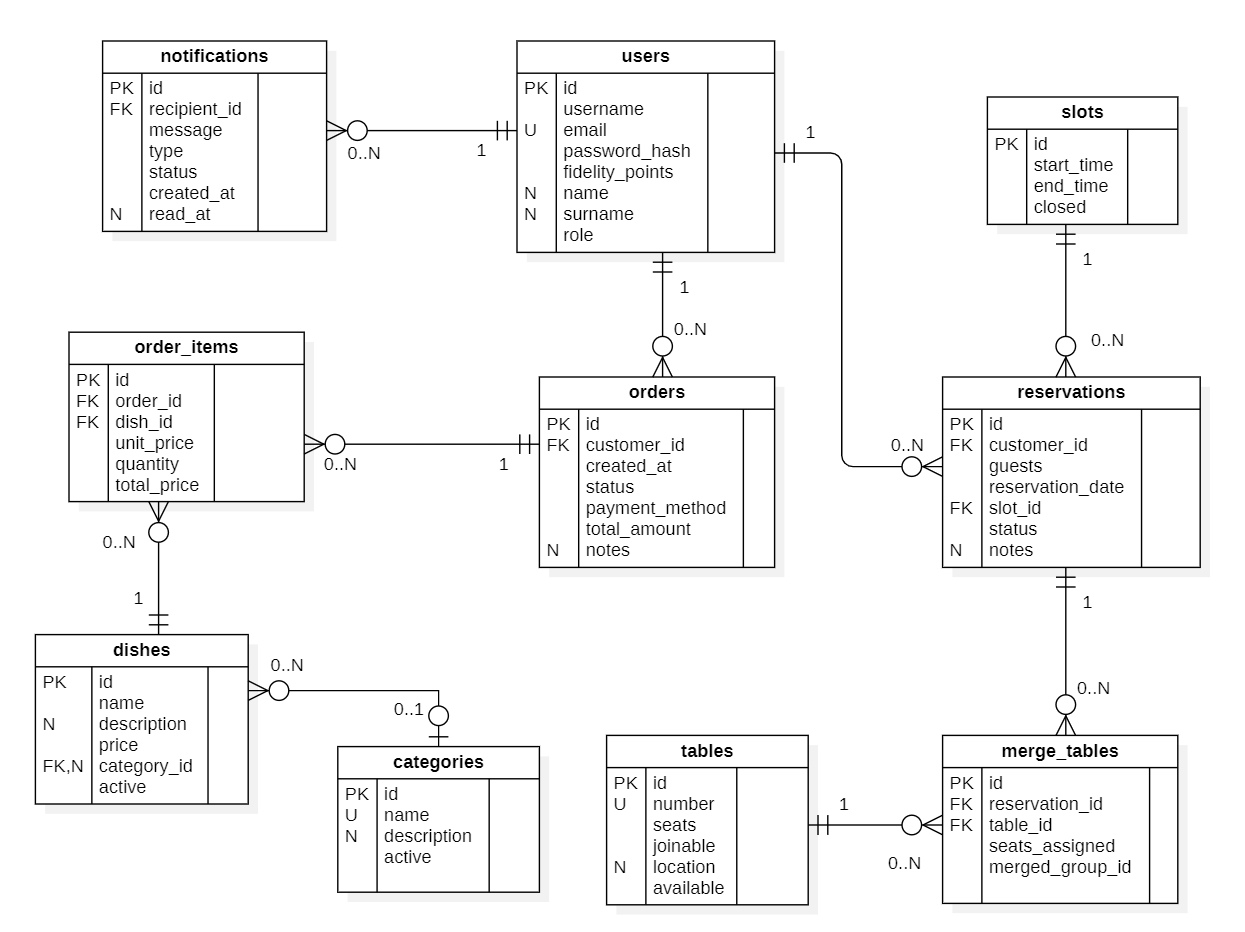
\includegraphics[width=\textwidth]{uml-diagramma-er.png}
  \caption{Diagramma Entity--Relationship del database DineUp.}
  \label{fig:database}
\end{figure}

Lo schema comprende dieci tabelle:
\code{users}, \code{categories}, \code{dishes}, \code{tables}, \code{slots},
\code{reservations}, \code{orders}, \code{order\_items},
\code{notifications} e \code{merge\_tables}. I vincoli \code{CHECK} replicano
nel database le condizioni fondamentali del dominio: quantità e prezzi non
negativi, numero di ospiti positivo, valori ammessi per ruoli e stati.

Nel diagramma, \code{PK} identifica le chiavi primarie, \code{FK} le chiavi
esterne, \code{U} i vincoli di unicità e \code{N} gli attributi nullable.
\code{merge\_tables} risolve la relazione molti-a-molti tra prenotazioni e
tavoli e conserva i posti assegnati e l'identificativo del gruppo di tavoli
uniti. \code{order\_items} svolge un ruolo analogo tra ordini e piatti,
memorizzando quantità e prezzo unitario storico.

\subsection{Traduzione nel modello relazionale}

Il modello relazionale separa le entità principali dalle associazioni che
possiedono attributi propri. \code{order\_items}, per esempio, non rappresenta
soltanto il collegamento tra ordine e piatto: conserva quantità e prezzo al
momento dell'acquisto. Allo stesso modo \code{merge\_tables} memorizza i posti
assegnati e l'identificativo del gruppo di tavoli uniti.

\begin{longtable}{p{3.2cm}p{10.6cm}}
\caption{Responsabilità delle tabelle del database.}\label{tab:db-tables}\\
\toprule
\textbf{Tabella} & \textbf{Responsabilità} \\
\midrule
\endfirsthead
\toprule
\textbf{Tabella} & \textbf{Responsabilità} \\
\midrule
\endhead
\code{users} & Account, credenziali cifrate, ruolo e punti fedeltà. \\
\code{categories} & Classificazione dei piatti e relativa visibilità. \\
\code{dishes} & Informazioni del menu, prezzo, disponibilità e categoria. \\
\code{tables} & Tavoli fisici, capienza, posizione e possibilità di unione. \\
\code{slots} & Fasce orarie utilizzabili per le prenotazioni. \\
\code{reservations} & Cliente, giorno, slot, numero di ospiti, stato e note. \\
\code{merge\_tables} & Assegnazione dei tavoli a una prenotazione. \\
\code{orders} & Testata dell'ordine, pagamento, importo totale e stato. \\
\code{order\_items} & Righe dell'ordine con quantità e prezzo unitario storico. \\
\code{notifications} & Messaggi destinati agli utenti e relativo stato di lettura. \\
\bottomrule
\end{longtable}

\subsection{Cardinalità e integrità referenziale}

Un utente può possedere più ordini, prenotazioni e notifiche; ciascuna di queste
occorrenze appartiene invece a un solo utente. Una categoria può classificare
più piatti, mentre il riferimento del piatto è opzionale perché
\code{category\_id} utilizza \code{ON DELETE SET NULL}. Un ordine contiene
zero o più righe e ciascuna riga fa riferimento a un piatto. Prenotazioni e
tavoli sono collegati attraverso \code{merge\_tables}, realizzando una
relazione molti-a-molti.

\begin{table}[H]
\centering
\rowcolors{2}{gray!8}{white}
\begin{tabular}{p{3.8cm}p{3.8cm}p{5.8cm}}
\toprule
\textbf{Chiave esterna} & \textbf{Riferimento} & \textbf{Cancellazione} \\
\midrule
\code{dishes.category\_id} & \code{categories.id} & Il riferimento diventa nullo con \code{SET NULL}. \\
\code{orders.customer\_id} & \code{users.id} & Impedita se l'utente possiede ordini. \\
\code{reservations.customer\_id} & \code{users.id} & Impedita se esistono prenotazioni. \\
\code{reservations.slot\_id} & \code{slots.id} & Impedita se lo slot è utilizzato. \\
\code{order\_items.order\_id} & \code{orders.id} & Le righe vengono eliminate con \code{CASCADE}. \\
\code{order\_items.dish\_id} & \code{dishes.id} & Impedita se il piatto è nello storico. \\
\code{notifications.recipient\_id} & \code{users.id} & Impedita se esistono notifiche. \\
\code{merge\_tables.reservation\_id} & \code{reservations.id} & Le assegnazioni vengono eliminate con \code{CASCADE}. \\
\code{merge\_tables.table\_id} & \code{tables.id} & Impedita se il tavolo è assegnato. \\
\bottomrule
\end{tabular}
\caption{Vincoli referenziali principali.}
\end{table}

Queste scelte proteggono lo storico: un piatto già ordinato o un tavolo già
utilizzato non può essere eliminato lasciando riferimenti non validi. Le entità
strettamente dipendenti, come righe d'ordine e assegnazioni dei tavoli, vengono
invece rimosse insieme al rispettivo aggregato.

\subsection{Vincoli di dominio nel database}

Le validazioni più importanti sono replicate anche nel database, così la
consistenza non dipende esclusivamente dal codice Java:

\begin{itemize}[leftmargin=*]
  \item email, nomi delle categorie e numeri dei tavoli sono univoci;
  \item prezzo, totale e punti fedeltà non possono essere negativi;
  \item quantità, capienza, ospiti e posti assegnati devono essere positivi;
  \item l'inizio di uno slot deve precederne la fine;
  \item ruoli, stati e metodi di pagamento appartengono a insiemi chiusi;
  \item \code{total\_price} viene calcolato dal database come
        \code{unit\_price * quantity}.
\end{itemize}

\begin{lstlisting}[style=codeStyle,language=SQL,
caption={Vincoli e colonna calcolata delle righe d'ordine.}]
CREATE TABLE order_items (
    id          SERIAL PRIMARY KEY,
    order_id    INT NOT NULL
                REFERENCES orders(id) ON DELETE CASCADE,
    dish_id     INT NOT NULL REFERENCES dishes(id),
    unit_price  NUMERIC(10,2) NOT NULL CHECK (unit_price >= 0),
    quantity    INT NOT NULL CHECK (quantity > 0),
    total_price NUMERIC(10,2)
                GENERATED ALWAYS AS (unit_price * quantity) STORED
);
\end{lstlisting}

Il prezzo unitario viene copiato nella riga invece di essere riletto da
\code{dishes}. In questo modo una variazione futura del menu non modifica il
valore economico degli ordini già conclusi.

\subsection{Accesso tramite JDBC e connection pool}

La persistenza è implementata senza framework ORM automatici. Ogni DAO estende
\code{BaseDAO} e utilizza JDBC con \code{PreparedStatement}, mantenendo
espliciti query e mapping. \code{DBConnection} configura un
\code{PGPoolingDataSource} condiviso attraverso il pattern Singleton:

\begin{lstlisting}[style=codeStyle,language=Java,
caption={Configurazione del pool di connessioni PostgreSQL.}]
PGPoolingDataSource ds = new PGPoolingDataSource();
ds.setDataSourceName("dineup-pool");
ds.setUrl(url);
ds.setUser(user);
ds.setPassword(password);
ds.setCurrentSchema(schema);
ds.setInitialConnections(4);
ds.setMaxConnections(20);
\end{lstlisting}

URL, utente e password vengono letti, in ordine di priorità, da proprietà di
sistema, variabili d'ambiente oppure file \code{db.properties}. Le credenziali
locali non sono versionate. Quando una connessione viene prelevata dal pool,
l'applicazione reimposta inoltre il \code{search\_path}: ciò impedisce che una
sessione riutilizzata conservi lo schema selezionato da un'operazione precedente
o da un test di integrazione.

\subsection{Mapping tra SQL e Domain Model}

I DAO trasformano i valori relazionali in oggetti di dominio. Le enumerazioni
sono memorizzate attraverso il relativo nome, gli importi vengono ricostruiti
come \code{Money} e le date SQL vengono convertite nei tipi
\code{java.time}. Le associazioni non necessarie al caso d'uso sono
rappresentate inizialmente mediante oggetti contenenti il solo identificativo,
evitando caricamenti indiscriminati.

\begin{lstlisting}[style=codeStyle,language=Java,
caption={Esempio di mapping di una riga della tabella orders.}]
Order order = new Order();
order.setId(rs.getInt("id"));

User customer = new User();
customer.setId(rs.getInt("customer_id"));
order.setCustomer(customer);

order.setCreatedAt(rs.getTimestamp("created_at").toLocalDateTime());
order.setStatus(OrderStatus.valueOf(rs.getString("status")));
order.setTotalAmount(new Money(rs.getBigDecimal("total_amount")));
\end{lstlisting}

Tutte le risorse JDBC sono racchiuse in blocchi
\emph{try-with-resources}. I parametri non vengono concatenati nelle query, ma
associati ai placeholder, riducendo il rischio di SQL injection e gli errori di
conversione.

\subsection{Transazioni atomiche}

Ordine e righe d'ordine devono essere salvati insieme. Se una singola riga
fallisce, anche l'ordine viene annullato:

\begin{lstlisting}[style=codeStyle,language=Java,
caption={Transazione per ordine e righe.}]
conn.setAutoCommit(false);
try {
    insertOrder(conn, order);
    insertOrderItems(conn, order.getId(), items);
    conn.commit();
} catch (SQLException | RuntimeException e) {
    conn.rollback();
    throw e;
}
\end{lstlisting}

La stessa proprietà viene garantita per prenotazione e assegnazioni dei tavoli
da \code{ReservationDAO.addReservationWithTables()}.

\subsection{Prevenzione delle doppie prenotazioni}

Un controllo effettuato soltanto dal Service Layer non sarebbe sufficiente in
presenza di richieste concorrenti. La migrazione
\code{V2\_\_prevent\_double\_table\_booking.sql} introduce un trigger che:

\begin{enumerate}[leftmargin=*]
  \item recupera giorno e slot della prenotazione;
  \item acquisisce un advisory lock transazionale per quella coppia;
  \item verifica se il tavolo è già associato a una prenotazione attiva;
  \item rifiuta l'inserimento in caso di conflitto.
\end{enumerate}

La protezione è quindi applicata sia a livello applicativo sia nel punto ultimo
di consistenza, il database.

\begin{lstlisting}[style=codeStyle,language=SQL,
caption={Controllo concorrente contro la doppia prenotazione.}]
PERFORM pg_advisory_xact_lock(
    hashtextextended(booking_date::TEXT || ':' ||
                     booking_slot::TEXT, 0)
);

IF EXISTS (
    SELECT 1
    FROM merge_tables mt
    JOIN reservations r ON r.id = mt.reservation_id
    WHERE mt.table_id = NEW.table_id
      AND r.reservation_date = booking_date
      AND r.slot_id = booking_slot
      AND r.status NOT IN ('CANCELED', 'NO_SHOW', 'COMPLETED')
) THEN
    RAISE EXCEPTION 'Table already booked';
END IF;
\end{lstlisting}

L'advisory lock serializza le assegnazioni relative alla stessa data e allo
stesso slot. Il controllo viene quindi eseguito senza la classica finestra di
gara tra lettura della disponibilità e successivo inserimento.

\subsection{Indici e prestazioni}

Il trigger e le query di disponibilità consultano frequentemente giorno, slot,
stato e tavolo. Per evitare scansioni complete sono definiti due indici
composti:

\begin{lstlisting}[style=codeStyle,language=SQL,
caption={Indici a supporto delle prenotazioni.}]
CREATE INDEX idx_reservations_date_slot_status
    ON reservations(reservation_date, slot_id, status);

CREATE INDEX idx_merge_tables_table_reservation
    ON merge_tables(table_id, reservation_id);
\end{lstlisting}

Il primo accelera la selezione delle prenotazioni attive per giorno e fascia
oraria; il secondo supporta il controllo delle assegnazioni di un tavolo. Le
chiavi primarie e i vincoli \code{UNIQUE} generano inoltre automaticamente gli
indici necessari per identificativi, email, categoria e numero del tavolo.

\subsection{Migrazioni}

Lo schema iniziale è contenuto in \code{sql/schema.sql}; il file
\code{sql/seed.sql} inserisce dati dimostrativi per tutti i ruoli e per le
principali entità. Le modifiche successive sono conservate in file numerati e
applicabili tramite \code{DatabaseMigrator}. Il progetto include:

\begin{itemize}[leftmargin=*]
  \item \code{V2\_\_prevent\_double\_table\_booking.sql}, che installa
        funzione, trigger e indici per la concorrenza;
  \item \code{V3\_\_normalize\_legacy\_notification\_types.sql}, che converte
  tipologie storiche non più previste;
  \item \code{V4\_\_normalize\_legacy\_notification\_statuses.sql}, che
  normalizza gli stati delle notifiche.
\end{itemize}

\code{DatabaseMigrator} consente di eseguire una migrazione SQL utilizzando la
stessa configurazione JDBC dell'applicazione. La numerazione rende esplicito
l'ordine di applicazione e permette di ricostruire l'evoluzione dello schema.
Le migrazioni V3 e V4 sono operazioni di pulizia dei dati e non modificano il
diagramma Entity--Relationship.

\section{Implementazione dei livelli}

\subsection{CLI}

Le CLI sono divise per ruolo. \code{Main} gestisce login, registrazione e reset
della password; dopo l'autenticazione effettua il dispatch verso
\code{CustomerCLI}, \code{StaffCLI} o \code{OwnerCLI}. Le operazioni private
delle CLI si occupano esclusivamente di acquisire dati, chiamare il Controller e
stampare il risultato.

\begin{lstlisting}[style=codeStyle,language=Java,
caption={La CLI gestisce input e output, delegando il caso d'uso.}]
private void handleCheckout(User user) {
    PaymentMethod method = readPaymentMethod();
    if (method == null) return;
    System.out.print("Note (facoltative): ");
    String notes = scanner.nextLine().trim();

    try {
        Order order = customerController.checkoutTakeAway(
            user, method, notes.isBlank() ? null : notes);
        System.out.println("Ordine creato con ID " + order.getId());
    } catch (SQLException | IllegalArgumentException
             | IllegalStateException e) {
        System.err.println("Errore: " + e.getMessage());
    }
}
\end{lstlisting}

\subsection{Controller}

\begin{table}[H]
\centering
\rowcolors{2}{gray!8}{white}
\begin{tabular}{p{4.4cm}p{9.6cm}}
\toprule
\textbf{Controller} & \textbf{Responsabilità} \\
\midrule
\code{AuthController} & Login, registrazione Customer e reset password. \\
\code{CustomerController} & Menu, ricerca, carrello, checkout, prenotazioni e notifiche. \\
\code{CustomerProfile}\newline\code{Controller} & Lettura e modifica del profilo. \\
\code{StaffController} & Coda cucina, stati ordine, prenotazioni, ricerca e notifiche. \\
\code{OwnerController} & Amministrazione delle risorse, ricerca e notifiche. \\
\bottomrule
\end{tabular}
\caption{Controller applicativi.}
\end{table}

\begin{lstlisting}[style=codeStyle,language=Java,
caption={Coordinamento del checkout nel CustomerController.}]
public Order checkoutTakeAway(User user,
                               PaymentMethod paymentMethod,
                               String notes) throws SQLException {
    List<OrderItem> items = cartService.getCartItems(user);
    if (items.isEmpty()) {
        throw new IllegalStateException("Il carrello e' vuoto");
    }

    Order order = orderService.placeTakeAwayOrder(
        user, items, paymentMethod, notes);
    cartService.clearCart(user);
    return order;
}
\end{lstlisting}

Il Controller orchestra più servizi ma non esegue stampe e non contiene SQL.
Il carrello viene svuotato soltanto dopo il completamento del salvataggio
dell'ordine.

\subsection{Servizi}

I servizi principali sono:

\begin{itemize}[leftmargin=*]
  \item \code{AuthService}, per autenticazione e hashing delle password;
  \item \code{CartService}, per il carrello in memoria;
  \item \code{MenuQueryService}, per menu e piatti;
  \item \code{OrderService} e \code{ReservationService}, per i due flussi
        transazionali centrali;
  \item \code{TableAllocationService}, per la combinazione dei tavoli;
  \item \code{OwnerAdminService} e \code{StaffOperationService}, per i casi
        d'uso specifici dei ruoli;
  \item \code{NotificationService}, \code{ProfileService} e
         \code{SearchService}.
\end{itemize}

Il metodo seguente esemplifica il ruolo del Service Layer: applica le
precondizioni del caso d'uso, coordina più collaboratori e costruisce le entità
di dominio, lasciando al DAO la persistenza atomica. In particolare, una
prenotazione viene accettata soltanto se lo slot è aperto e se
\code{TableAllocationService} individua una combinazione di tavoli sufficiente.

\begin{lstlisting}[style=codeStyle,language=Java,
caption={Coordinamento della creazione di una prenotazione nel Service Layer.}]
Slot slot = slotDAO.getSlotById(slotId)
    .orElseThrow(() ->
        new IllegalArgumentException("Slot not found: " + slotId));
if (slot.isClosed()) {
    throw new IllegalStateException("Selected slot is closed");
}

Set<Integer> reserved = new HashSet<>(
    reservationDAO.getReservedTableIds(date, slotId));
List<Table> available = tableDAO.getAvailableTables().stream()
    .filter(table -> !reserved.contains(table.getId()))
    .toList();

List<Table> combination =
    tableAllocationService.findBestCombination(available, guests);
if (combination == null || combination.isEmpty()) {
    throw new IllegalStateException(
        "No tables available for the requested slot");
}

Reservation reservation = new Reservation(
    customer, LocalDateTime.of(date, slot.getStartTime()),
    slot, guests, notes);
List<MergeTable> assignments =
    reservationDAO.addReservationWithTables(reservation, combination);
reservation.setTables(assignments);
return reservation;
\end{lstlisting}

\subsection{Autenticazione e protezione delle password}

\code{AuthService} valida gli input, recupera l'utente tramite DAO e delega a
BCrypt la verifica della password. In fase di registrazione e modifica non viene
mai salvata la password in chiaro.

\begin{lstlisting}[style=codeStyle,language=Java,
caption={Hashing e verifica delle password con BCrypt.}]
Optional<User> maybeUser = userDAO.getUserByEmail(email);
if (maybeUser.isEmpty()) {
    return Optional.empty();
}

User user = maybeUser.get();
if (!BCrypt.checkpw(rawPassword, user.getPasswordHash())) {
    return Optional.empty();
}
return Optional.of(user);

// Registrazione o cambio password
String hash = BCrypt.hashpw(rawPassword, BCrypt.gensalt());
\end{lstlisting}

\section{Prototipazione dell'interfaccia grafica}

\subsection{Finalità e provenienza dei mockup}

L'applicazione realizzata utilizza un'interfaccia a riga di comando. Per
mostrare come la medesima architettura potrebbe essere riutilizzata da una
successiva interfaccia web, sono stati progettati alcuni mockup ad alta
fedeltà.

I mockup rappresentano una possibile evoluzione grafica dell'applicazione
\project{}. Le schermate includono sia le funzionalità implementate nel
prototipo Java a riga di comando, sia alcune estensioni previste per una futura
versione completa. Grafici, indicatori economici e dati riepilogativi sono
dimostrativi e non rappresentano risultati prodotti dall'implementazione
attuale.

I mockup sono stati progettati dagli autori sulla base dei requisiti e dei casi
d'uso del sistema e realizzati con il supporto dello strumento generativo
ChatGPT di OpenAI, tramite l'integrazione con Canva. Le immagini costituiscono
prototipi grafici e non schermate dell'applicazione attualmente implementata.

\subsection{Accesso e registrazione}

Le schermate di accesso riprendono i casi d'uso offerti da
\code{AuthController}: autenticazione, registrazione del Customer e recupero
della password. I ruoli Staff e Owner non possono registrarsi autonomamente;
l'assegnazione del ruolo determina soltanto la dashboard aperta dopo il login.

\begin{figure}[H]
  \centering
  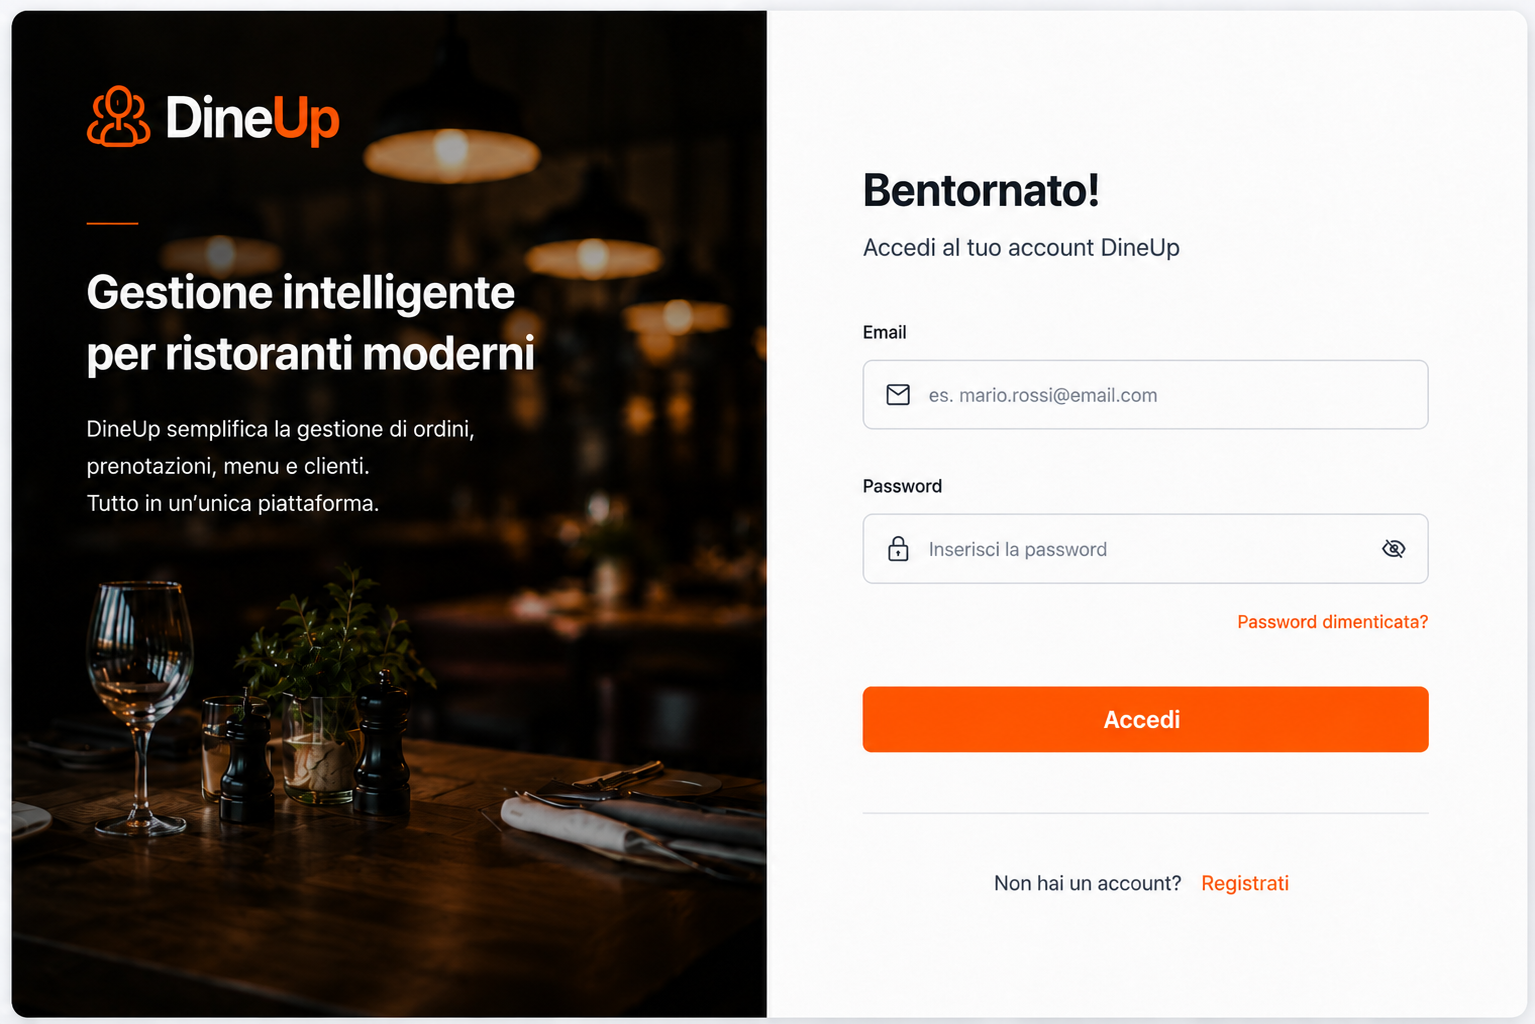
\includegraphics[width=0.74\textwidth]{mokup/login3.png}
  \caption{Mockup della schermata di autenticazione.}
  \label{fig:mockup-login}
\end{figure}

\begin{figure}[H]
  \centering
  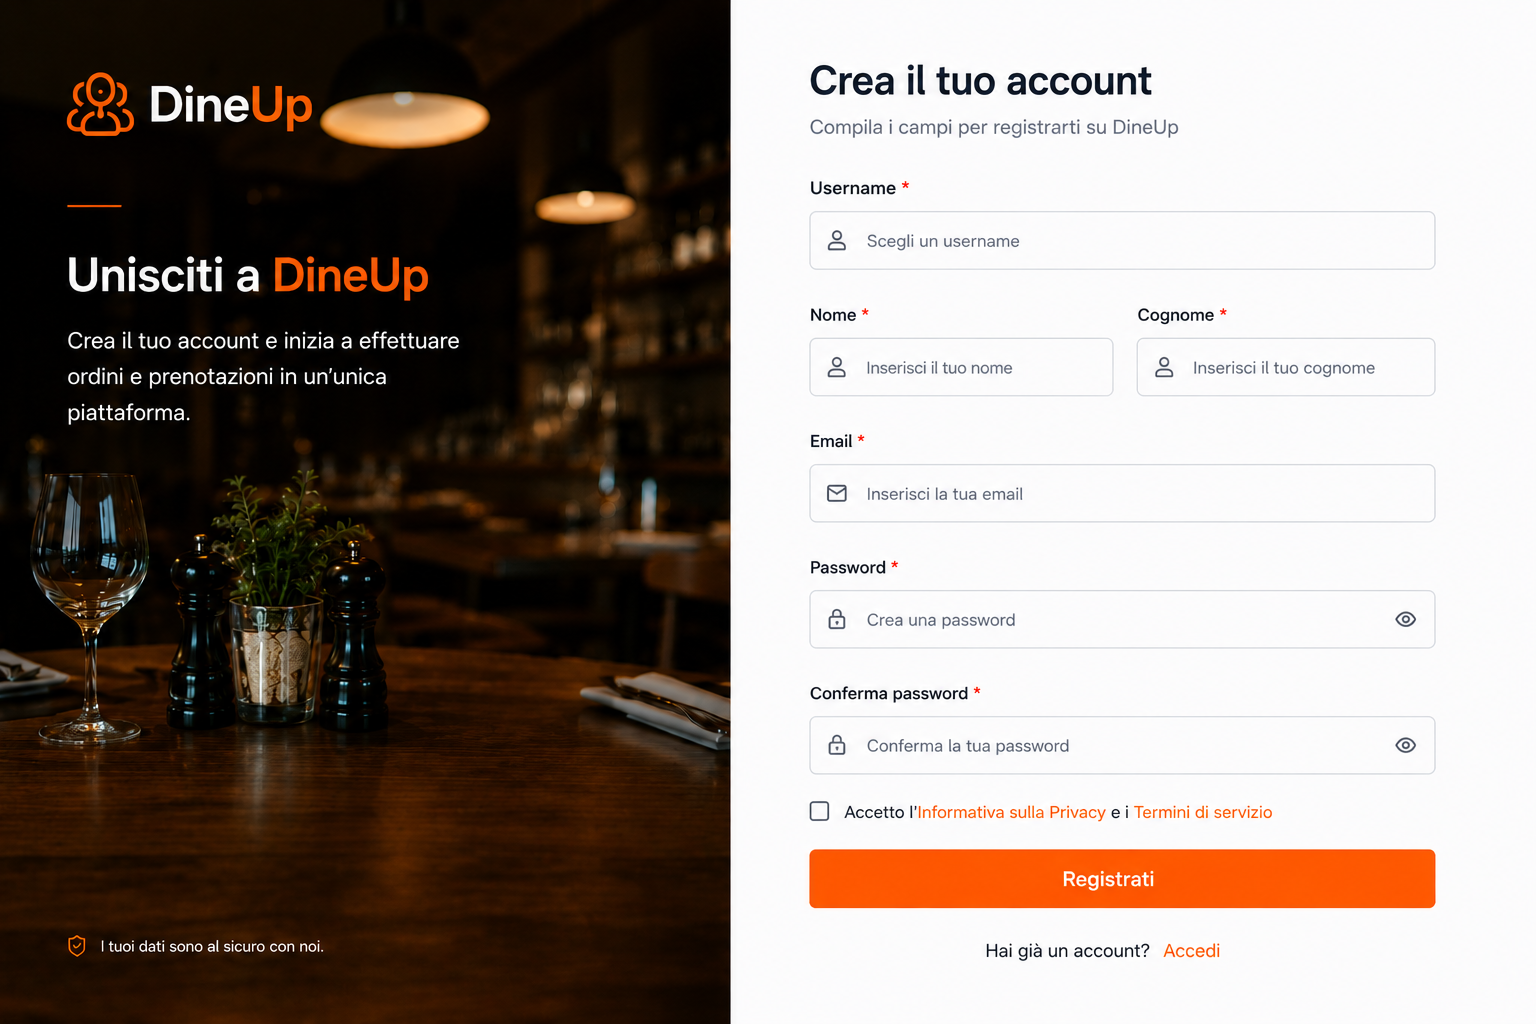
\includegraphics[width=0.74\textwidth]{mokup/registrazione3.png}
  \caption{Mockup della registrazione di un nuovo Customer.}
  \label{fig:mockup-register}
\end{figure}

\subsection{Dashboard Customer}

La dashboard del Customer riunisce menu, carrello, ordini d'asporto,
prenotazioni, notifiche e profilo. Il pagamento mostrato è esclusivamente al
ritiro; l'applicazione registra infatti la modalità di pagamento senza
integrare un gateway esterno. I promemoria rappresentano una possibile
estensione della gestione delle notifiche già presente.

\begin{figure}[H]
  \centering
  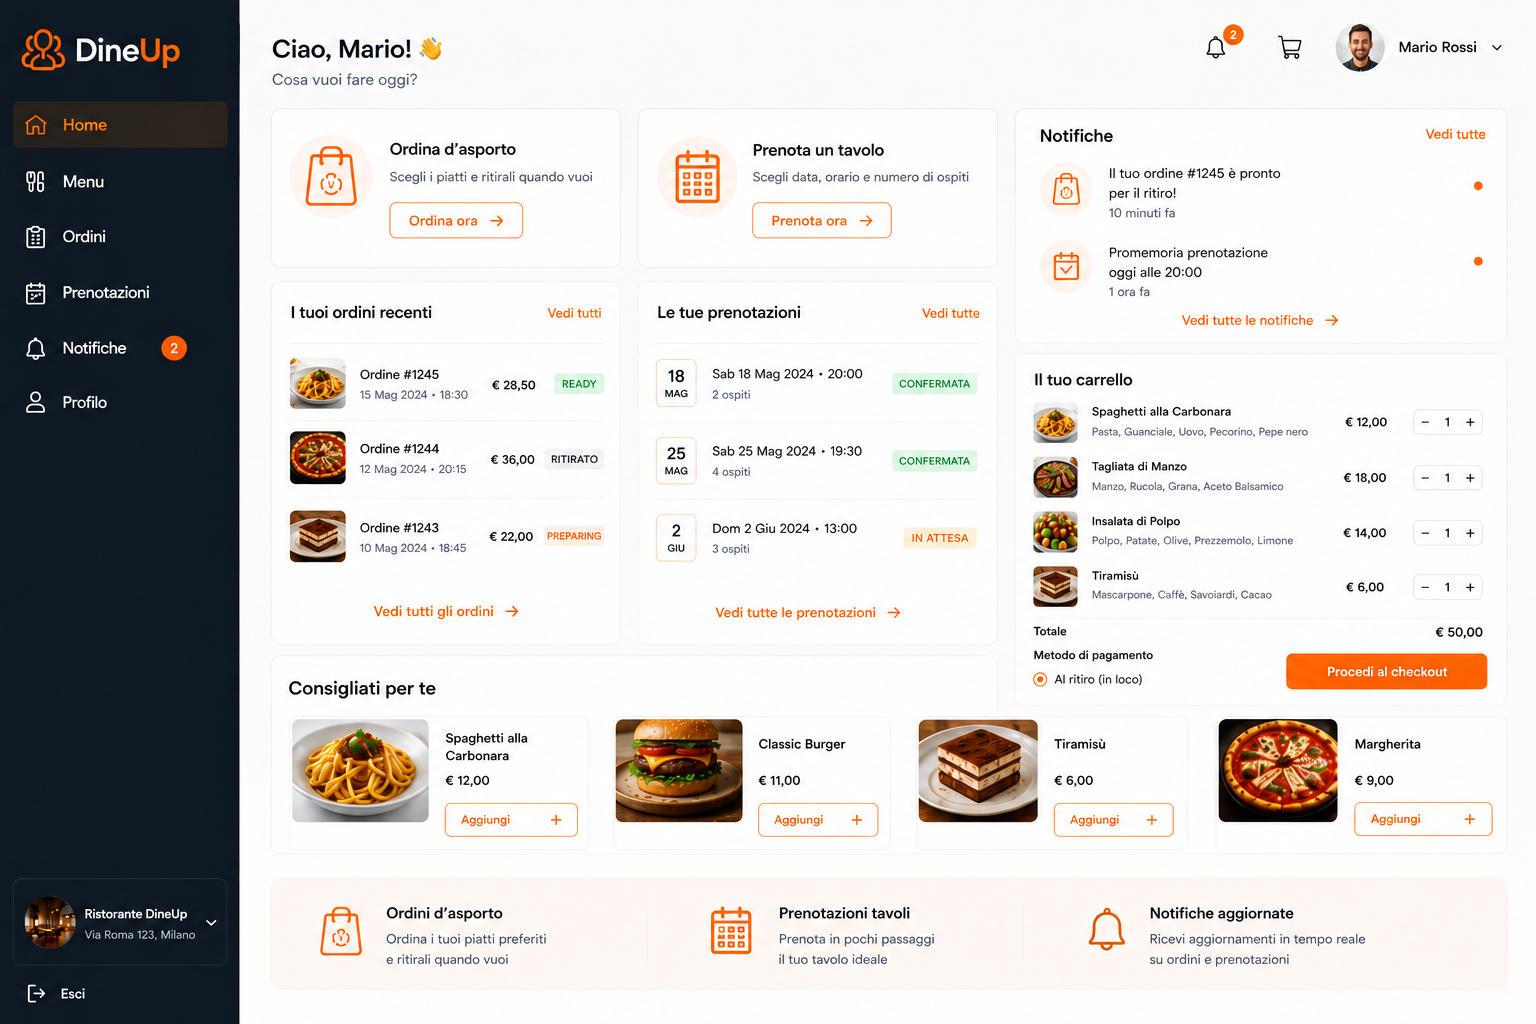
\includegraphics[width=\textwidth]{mokup/DashboardUser3.png}
  \caption{Mockup della dashboard Customer.}
  \label{fig:mockup-customer}
\end{figure}

\subsection{Dashboard Staff}

La dashboard dello Staff traduce graficamente la coda cucina, le transizioni
degli ordini e la gestione operativa delle prenotazioni. Le azioni principali
sono conferma, check-in, no-show, ricerca e aggiornamento delle notifiche.
Il planning costituisce una diversa visualizzazione delle prenotazioni per
data già disponibili nel sistema; l'invio manuale di una notifica è previsto
come estensione dell'interfaccia.

\begin{figure}[H]
  \centering
  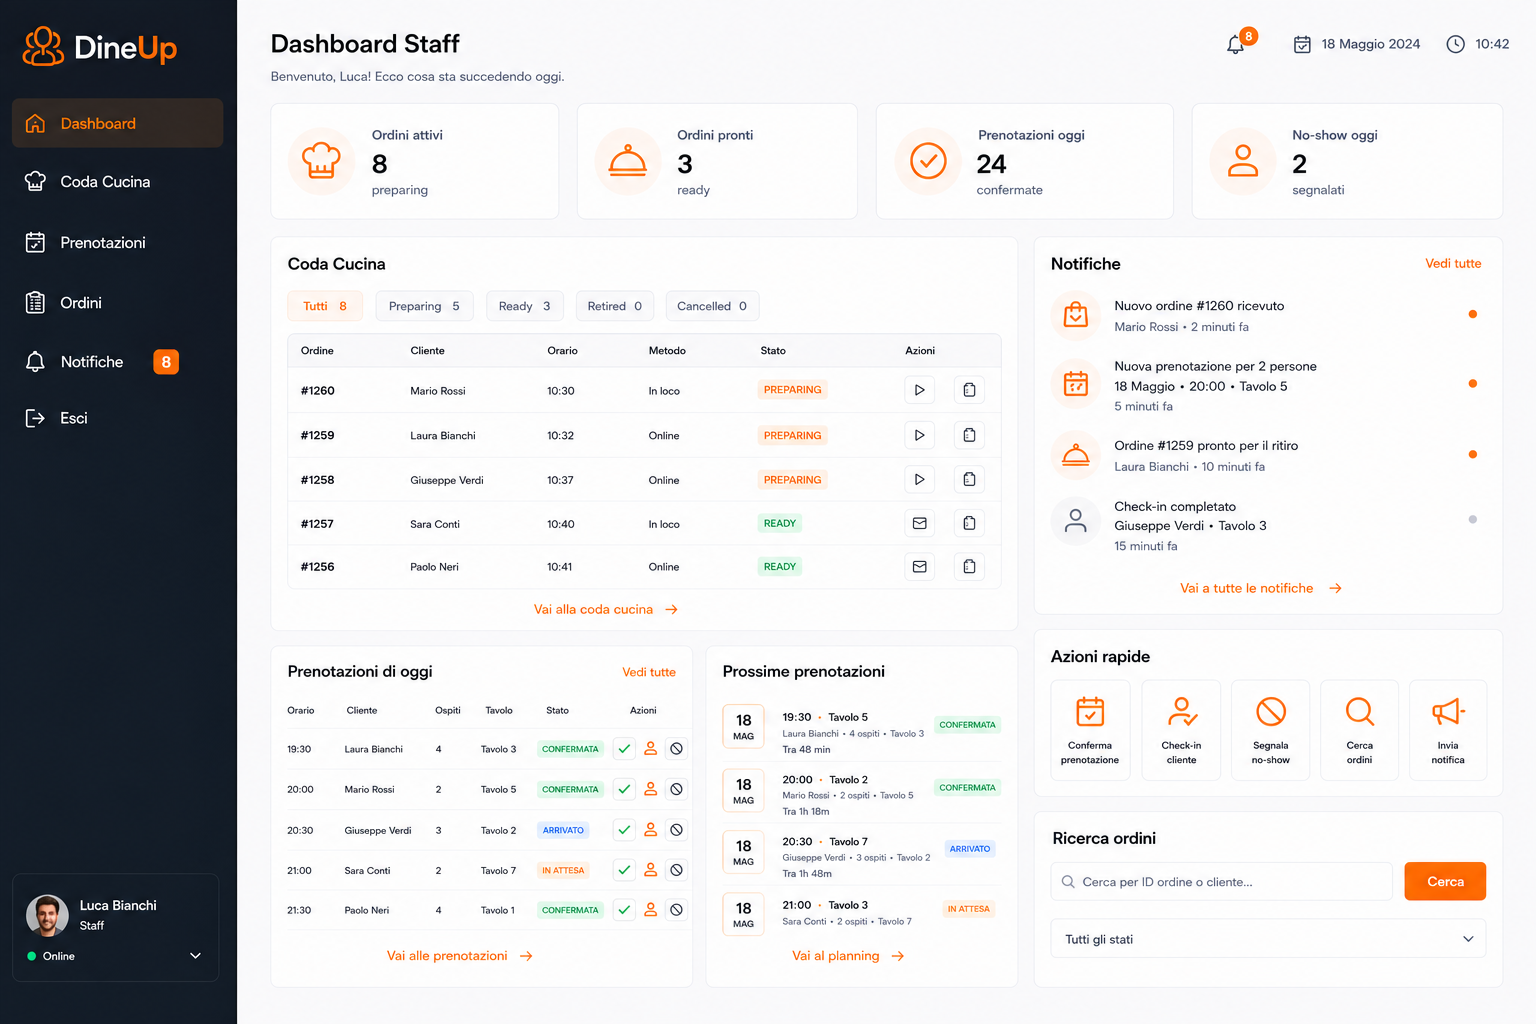
\includegraphics[width=\textwidth]{mokup/DashboardStaff3.png}
  \caption{Mockup della dashboard Staff.}
  \label{fig:mockup-staff}
\end{figure}

\subsection{Dashboard Owner}

La dashboard Owner raccoglie la gestione di menu, categorie, piatti, tavoli,
slot, ordini e prenotazioni. La creazione degli account Staff, le impostazioni
del ristorante, i report, l'esportazione e la modifica amministrativa dei flussi
sono evoluzioni previste. Fatturato, scontrino medio, confronti settimanali e
classifica dei piatti sono dati dimostrativi del prototipo grafico.

\begin{figure}[H]
  \centering
  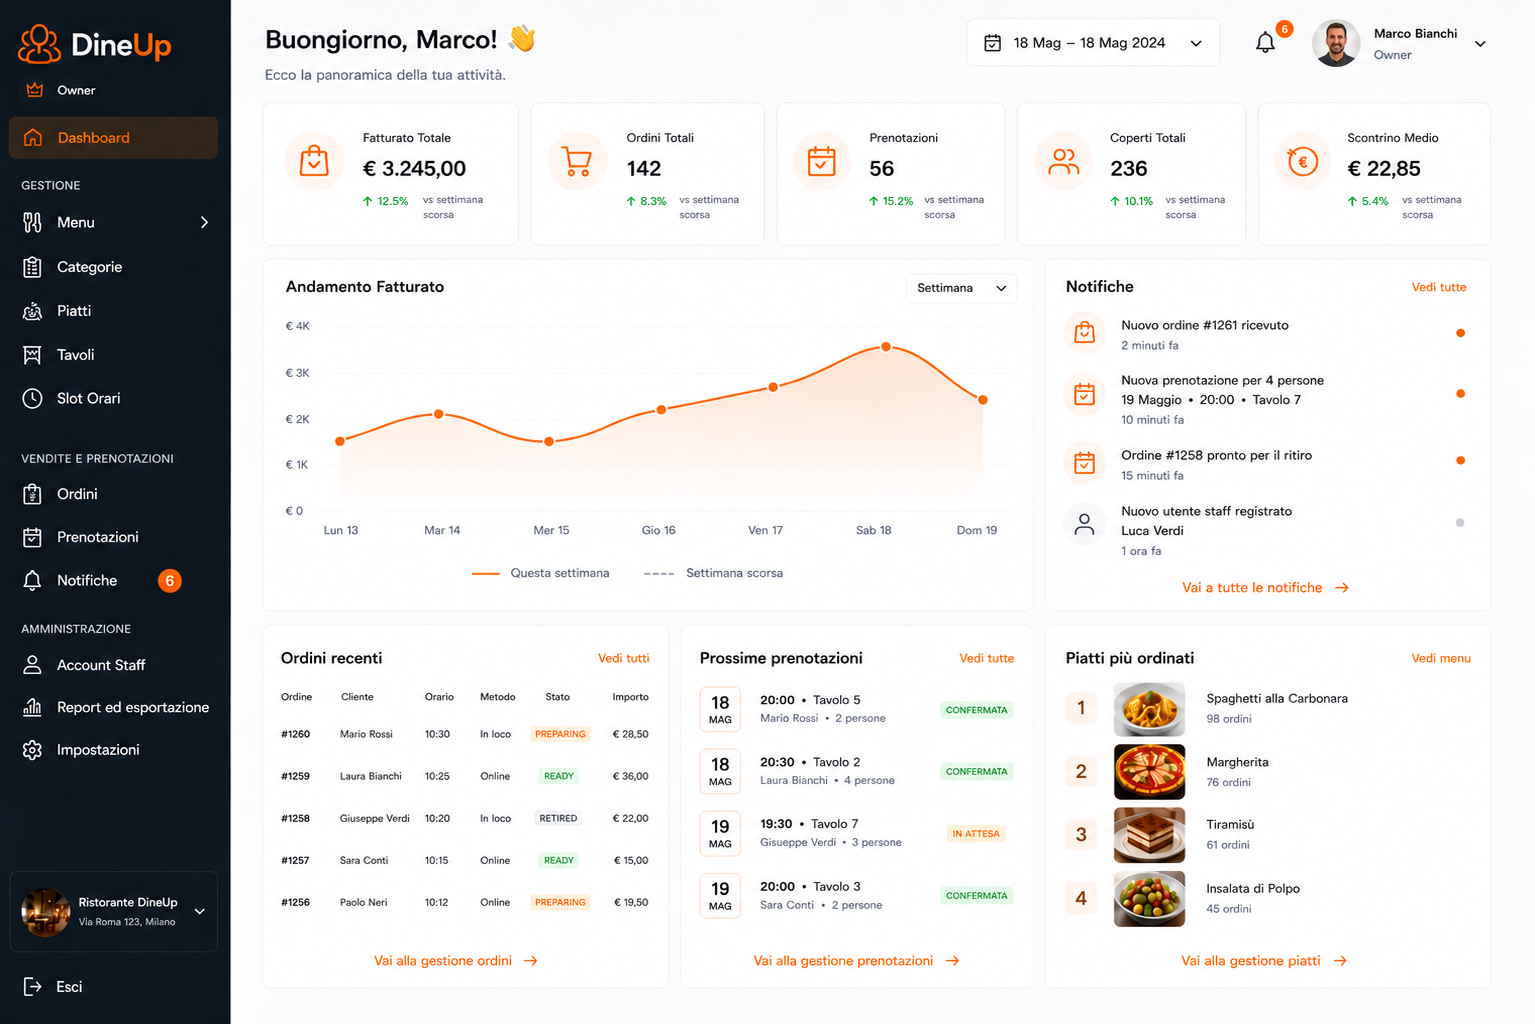
\includegraphics[width=\textwidth]{mokup/DashboardOwner3.png}
  \caption{Mockup della dashboard Owner.}
  \label{fig:mockup-owner}
\end{figure}

\section{Testing e validazione}

\subsection{Strategia}

La suite è organizzata in 16 classi e copre quattro livelli:

\begin{table}[H]
\centering
\begin{tabular}{p{3.6cm}p{10.4cm}}
\toprule
\textbf{Livello} & \textbf{Obiettivo} \\
\midrule
Domain Model & Validazioni, builder, criteri e risultati di ricerca. \\
Service Layer & Regole di business con collaboratori sostitutivi. \\
Controller & Verifica della delega e della composizione dei casi d'uso. \\
DAO Integration & Query reali, mapping, CRUD, transazioni, trigger e schema PostgreSQL. \\
\bottomrule
\end{tabular}
\caption{Livelli della strategia di test.}
\end{table}

\subsection{Test dei Service e dei Controller}

I servizi vengono testati isolando l'accesso ai dati. I test verificano sia i
flussi nominali sia le condizioni di errore: carrello vuoto, transizioni illegali,
prenotazioni senza tavoli disponibili, quantità non valide e dati mancanti.

Nei test dei Controller vengono utilizzate implementazioni \emph{fake} dei
servizi. Questo permette di controllare che ogni Controller:

\begin{itemize}[leftmargin=*]
  \item inoltri parametri e filtri corretti;
  \item restituisca il risultato del servizio senza trasformazioni improprie;
  \item coordini più servizi quando richiesto dal caso d'uso;
  \item non contenga logica di presentazione.
\end{itemize}

\begin{lstlisting}[style=codeStyle,language=Java,
caption={Test della politica di allocazione dei tavoli.}]
@Test
void findBestCombinationPrefersFewestTablesThenLeastWaste() {
    Table two = table(1, 2, true);
    Table four = table(2, 4, true);
    Table six = table(3, 6, false);

    List<Table> result =
        service.findBestCombination(List.of(two, four, six), 5);

    assertEquals(List.of(six), result);
}
\end{lstlisting}

Il test descrive una regola di business, non un dettaglio implementativo: un
tavolo singolo adatto deve essere preferito all'unione di più tavoli.

\subsection{Test di integrazione DAO}

\code{DaoIntegrationTest} crea uno schema PostgreSQL temporaneo dal nome casuale,
carica lo schema reale e configura l'applicazione affinché utilizzi esclusivamente
quello schema. Prima di ogni test le tabelle vengono svuotate; al termine lo
schema viene eliminato.

\begin{lstlisting}[style=codeStyle,language=Java,
caption={Isolamento dei test DAO mediante schema temporaneo.}]
private final String schema = "dineup_test_" +
    UUID.randomUUID().toString().replace("-", "");

statement.execute("CREATE SCHEMA " + schema);
statement.execute("SET search_path TO " + schema);
statement.execute(Files.readString(
    Path.of("sql", "schema.sql")));
\end{lstlisting}

La classe verifica tutti i DAO e comprende test dedicati a:

\begin{itemize}[leftmargin=*]
  \item CRUD e filtri dinamici;
  \item ordine con righe salvato atomicamente;
  \item prenotazione con assegnazioni tavoli;
  \item trigger contro la doppia prenotazione;
  \item transizioni delle notifiche;
  \item corretta impostazione dello schema nella connessione.
\end{itemize}

\begin{lstlisting}[style=codeStyle,language=Java,
caption={Test d'integrazione del trigger anti-doppia prenotazione.}]
reservationDAO.addReservationWithTables(
    new Reservation(customer, dateTime, slot, 2, null),
    List.of(table));

assertThrows(SQLException.class, () ->
    reservationDAO.addReservationWithTables(
        new Reservation(customer, dateTime, slot, 2, null),
        List.of(table)));
\end{lstlisting}

Questo test attraversa realmente DAO, JDBC, transazione e trigger PostgreSQL:
la seconda assegnazione equivalente deve fallire nel database.

\subsection{Esito}

L'esecuzione mediante \code{mvn clean test} termina con \textbf{91 test eseguiti},
\textbf{0 failure}, \textbf{0 error} e \textbf{0 test ignorati}. Il risultato è
stato verificato sull'ultima versione del progetto tramite Maven.

Oltre alla suite automatica sono stati effettuati test end-to-end manuali della
CLI per Customer, Staff e Owner, includendo l'interazione con il database reale.

\section{Sicurezza, affidabilità e gestione degli errori}

\begin{itemize}[leftmargin=*]
  \item Le password sono memorizzate come hash BCrypt.
  \item Le query utilizzano \code{PreparedStatement}.
  \item Le connessioni e gli statement sono chiusi con
        \emph{try-with-resources}.
  \item Le transazioni eseguono rollback in caso di errore.
  \item Il database impone vincoli di dominio e protegge dalla concorrenza.
  \item Le credenziali locali sono esterne al repository tramite
        \code{db.properties} ignorato da Git.
  \item CLI e Controller gestiscono gli errori senza esporre dettagli sensibili
        della configurazione.
\end{itemize}

\section{Conclusioni e sviluppi futuri}

\project{} realizza un gestionale console completo e verificato, con una chiara
separazione tra presentazione, casi d'uso, regole di business e persistenza. Le
scelte più significative sono l'uso di transazioni per gli aggregati, la
protezione database dalle doppie prenotazioni, i filtri Fluent Builder e una
suite di test che comprende anche il database reale.

Possibili evoluzioni sono:

\begin{itemize}[leftmargin=*]
  \item interfaccia grafica o applicazione web che riutilizzi Controller e servizi;
  \item autenticazione con sessioni e recupero password tramite canale esterno;
  \item modifica autonoma degli elementi di un ordine tramite
        \code{OrderItemDAO};
  \item politiche di allocazione tavoli configurabili;
  \item audit log delle operazioni amministrative;
  \item pipeline di integrazione continua.
\end{itemize}

\appendix

\section{Compilazione ed esecuzione}

\begin{lstlisting}[style=codeStyle,language=bash,
caption={Comandi Maven principali.}]
mvn clean test
mvn package
mvn exec:java
\end{lstlisting}

La configurazione del database può essere fornita mediante il file locale
\code{src/ORM/db.properties}, proprietà di sistema oppure variabili d'ambiente
\code{DB\_URL}, \code{DB\_USER} e \code{DB\_PASSWORD}.

\section{Repository}

\url{https://github.com/Cinotti02/swe_project}

\end{document}
